
\SB{In this work, the naming pattern of snoRNAs mostly follows the convention established by the original snoRNA sources. Normally, the predominant order of naming is: \emph{S.cerevisiae}, \emph{N.crassa}, \emph{A.fumigatus},
\emph{C.albicans}, and \emph{S.pombe}, i.e., snoRNA families are first of all 
adressed with their budding yeast name, in case there is no such
sequence in this particular family, the \emph{N.crassa} name will be
used, etc. In either way, the internal \snostrip -names will be given in parentheses. A complete mapping of \snostrip\ names with their species
specific names is shown in supplement S3. In case of target positions
we will denote the alignment position and the sequence specific
position of selected organisms are written in parentheses.}


\subsection{Expanded fungi snoRNA complement}

A set of 68 \cd\ and 50 \haca\ families were searched for additional homologs in 
147 fungal organisms. The U3 \sno\ family is considered separately due to its 
special function and characteristics and published elsewhere \cite{Canzler:2017}. All \snostrip\ retrieved snoRNA sequences 
were carefully cross-checked in all species to reduce the number of false 
negatives and exclude potentially wrong associations. This resulted in a total 
amount of 5595 and 2331 \cd\ and \haca\ sequences. Hence, we expanded the fungi 
snoRNA complement by \SB{XXX$\%$} and immensely increased its resolution. 

%Although, the characteristic box motifs C,D',C',D,H, and ACA, and the anti-sense 
%elements are highly conserved, the remaining sequence shows little or no 
%sequence conservation. In particular, the amount of not conserved nucleotides is 
%higher, hence the multiple sequence alignment algorithm is not always capable to 
%correctly align such sequences. We therefore anchored the sequences at their 
%conserved motifs and ASEs and recalculated the sequence alignment for the 
%remaining sequence. This procedure yielded reasonable alignments that could be 
%used for predicting a common secondary structure. \SB{What about 
%locarna?? $\rightarrow$ We decided against a combined sequence-structure 
%alignment approach (e.g. \locarna\citep{}) for two reasons: 1) our anchoring 
%procedure ensures to a hundred percent that we correctly align the ASEs and the 
%motifs which helps to identify a shared functional secondary structure, and 2) 
%the resulting alignments are still better than those produced with e.g. 
%locarna???} \SB{$\rightarrow$ Der ganze Absatz stoert mich irgendwie. So weit ich mich erinnern kann, konnte man nur mit locarna die sequencen an bestimmten positionen ankern. ( zumindest ohne grosse kofpstaende... diesen Ansatz haben wir aber im laufe der Zeit aufgegeben, hauptsaechlich weil mlocarna fuer HACAs so lange gerechnet hat. Muscle produzierte mindestens gleichwertige alignments in einem bruchteil der zeit. d.h. zur zeit werden die boxen NICHT geankert, sollten aber trotzdem aligniert werden. Um da sicher zu gehen dass die richtigen Boxen als boxen annotiert sind, gibt es ja diesen optionalen quality check. Ich denke ich wuerde auf die genaue alignment computation nicht weiter eingehen, die ganze pipeline ist ja schon im snoStrip paper erklaert, eigentlich sollte es reichen wenn man darauf verweist.....oder?}
%

\subsection{Observed fungi snoRNA characteristics}

\paragraph{\textbf{Box motifs}} Sequence motifs were created from all \snostrip-annotated \sno s. They can be downloaded from the supplement.
In general these motifs follow the propagated rules for canonical \sno\ box motifs known from yeast and animals: 

Box C (RUGAUGA) and D (CUGA) match the consensus sequence motifs
almost perfectly. Box C shows a purine (R) in 92\% of all cases. 
The 5' GA di-nucleotide is conserved to 100\%. 
The 5' nucleotide (C) of box D
shows few mutations (4.2\%) mostly towards an adenine while the
remaining positions are highly conserved ($\ge$99.7\%). 

As expected from yeast and other animal snoRNAs the situation is different for the prime box motifs. 
In box C', merely the 5' UG di-nucleotide and, to a lesser extent, the
trailing GA di-nucleotide show high conservation.
This might indicate a role in the binding of snoRNP associated proteins.
In box D' variations of the canonical nucleotides occur quite
frequently (between 15\% and 45\%) in each position.

In \haca s, we observe that the sequence of box ACA is highly conserved with
slight variations in its middle position. The adenine residues of box H (ANANNA) are highly conserved at the 1$^{st}$ and
3$^{rd}$ position while the trailing adenine (6$^{th}$ position) is more variable. The
2$^{nd}$ position of this motif is a guanine in nearly 80\% of the \haca s, whereas the other "N" associated positions (4$^{th}$ and 5$^{th}$ position) do not show a favoured nucleotide.

\paragraph{\textbf{Sequence}} \JH{Can we include a figure, e.g. boxplot for all boxes of \cd s and \haca s here? I don't like these numbers in the text.} In
accordance with the published \cd\ length, 90\% of the novel
\snostrip-annotated  \sno s are 80-135nt in length, with a median of 93nt (data not shown). 
Family Nc\_CD\_53 (\ncr, CD\_53 in \snostrip) is the only exception since its members share sequences with lengths between 200 and 300nt. 
Crucial features are the distances between box C
and the potential box D'  as well as between box C' and D
since these stretches harbor the target binding sites. 
Box C/D' distances are observed to be at least 11nt (median: 24nt), while box C'/D distances span at least 9nt (median: 22nt). 
The distance between boxes D' and C' is not known to be of significant relevance although at least 2nt are required to form another kink-turn motif supported by  the snoRNP associated proteins. 
Larger distances do not pose a problem there. 
Within the fungi \sno s, the shortest distance is 3nt while 80\% of all
prime box annotated sequences possess distance between 6 to 31
nucleotides.

Box H/ACA snoRNAs are reasonably longer. Their
median sequence length is 188nt. The shortest sequence comprises 115nt, while 90\% of all sequences are between 148 and 266nt. 
The lengths of both hairpin structures are similar: 85 and 79nt for hairpin 1 (HP1) and hairpin 2 (HP2), respectively. 
Extraordinary long
\sno s can be found in families snR86 (HACA\_36) and snR84 (HACA\_41)
with lengths of $\sim$1000nt and $\sim$600nt, respectively. Family
snR30 (HACA\_12), which is $\sim$600nt long, provides an exceptional
secondary structure with extensively enlarged 5' hairpins and hinge
regions, where the latter one is also able to form a so-called
internal hairpin \citep{Fayet-Lebaron:2009}.


\paragraph{\textbf{Structure}} Due to its specific
post-transcriptional processing by exonucleases, both trailing ends of
\cd s are cut not farther than 5 nucleotides apart from box C and D,
respectively \citep{Kishore:2013}. Owed to these rather short ends,
only a small subset of \sno\ sequences were predicted to fold a short closing stem (1208 out of 5595). 
If we enlarge the trailing ends to 10nt instead, a stem could be predicted for nearly 60\% (3317). 
These observations and the rather large fraction of \sno s that are still unable to fold into a characteristic stem loop structure indicate that a specific naturally occurring secondary structure is probably not needed for \cd s to fulfil their function. 
In consequence, snoRNP-associated proteins may take charge of bringing the RNA molecule and the assembled proteins into the correct functional conformation.

In contrast, \haca s are required to develop a significant and specific secondary structure to function appropriately. Only 15\% (395 out of 2269) of all snoRNAs were not predicted to fold into a stem-loop structure for both hairpins. 

In general, \sno -specific characteristics like box motifs, lengths,
and secondary structures are highly comparable between Fungi and
Metazoa \cite{Kehr:2014}. 


\subsection{Evolution of fungi snoRNAs}
  
\paragraph{\textbf{Phylogenetic distribution of snoRNAs}}
A heatmap depicting the distribution of  fungal \cd\ families is shown
in figure \ref{fig:heatmap_CD_snoRNAs}. A similar illustration of
\haca\ families can be seen in supplementary Figure S5. In both figures, the
amount of \sno\ sequences belonging to a particular organism and
family is color encoded.

\JH{Please rephrase the next paragraph}
In general, fungal \sno\ families encompass exactly one \sno\ sequence
per organism. Exceptions of this rule are given by 
families CD\_5 and CD\_19 whose coverage number mainly lies between two and
three. This is rather a technical result of how \snostrip\ works than a
detected biological event where snoRNA families contain mutliple
copies of the exact same \sno\ gene. Due to detected target
switches and target duplications \snostrip\ was promted to
automatically merge previously separate \sno\ familes and hence,
virtually increases the copy numbers. Details are explained
later when target switches are discussed. 

Besides an enlarged
\sno\ coverage in specific families, it frequently happens that
certain species encode an increased amount of paralogs to one or
many \sno\ families, e.g., \Ppl, \Asp\ or \Nfu. Even
whole lineages share increased copy numbers in certain families, e.g., 
Leotiomycetes in AM921940 (CD\_41) or Sordariomycetes in Nc\_CD\_28 (CD\_28).

\begin{figure*}
  \centering
  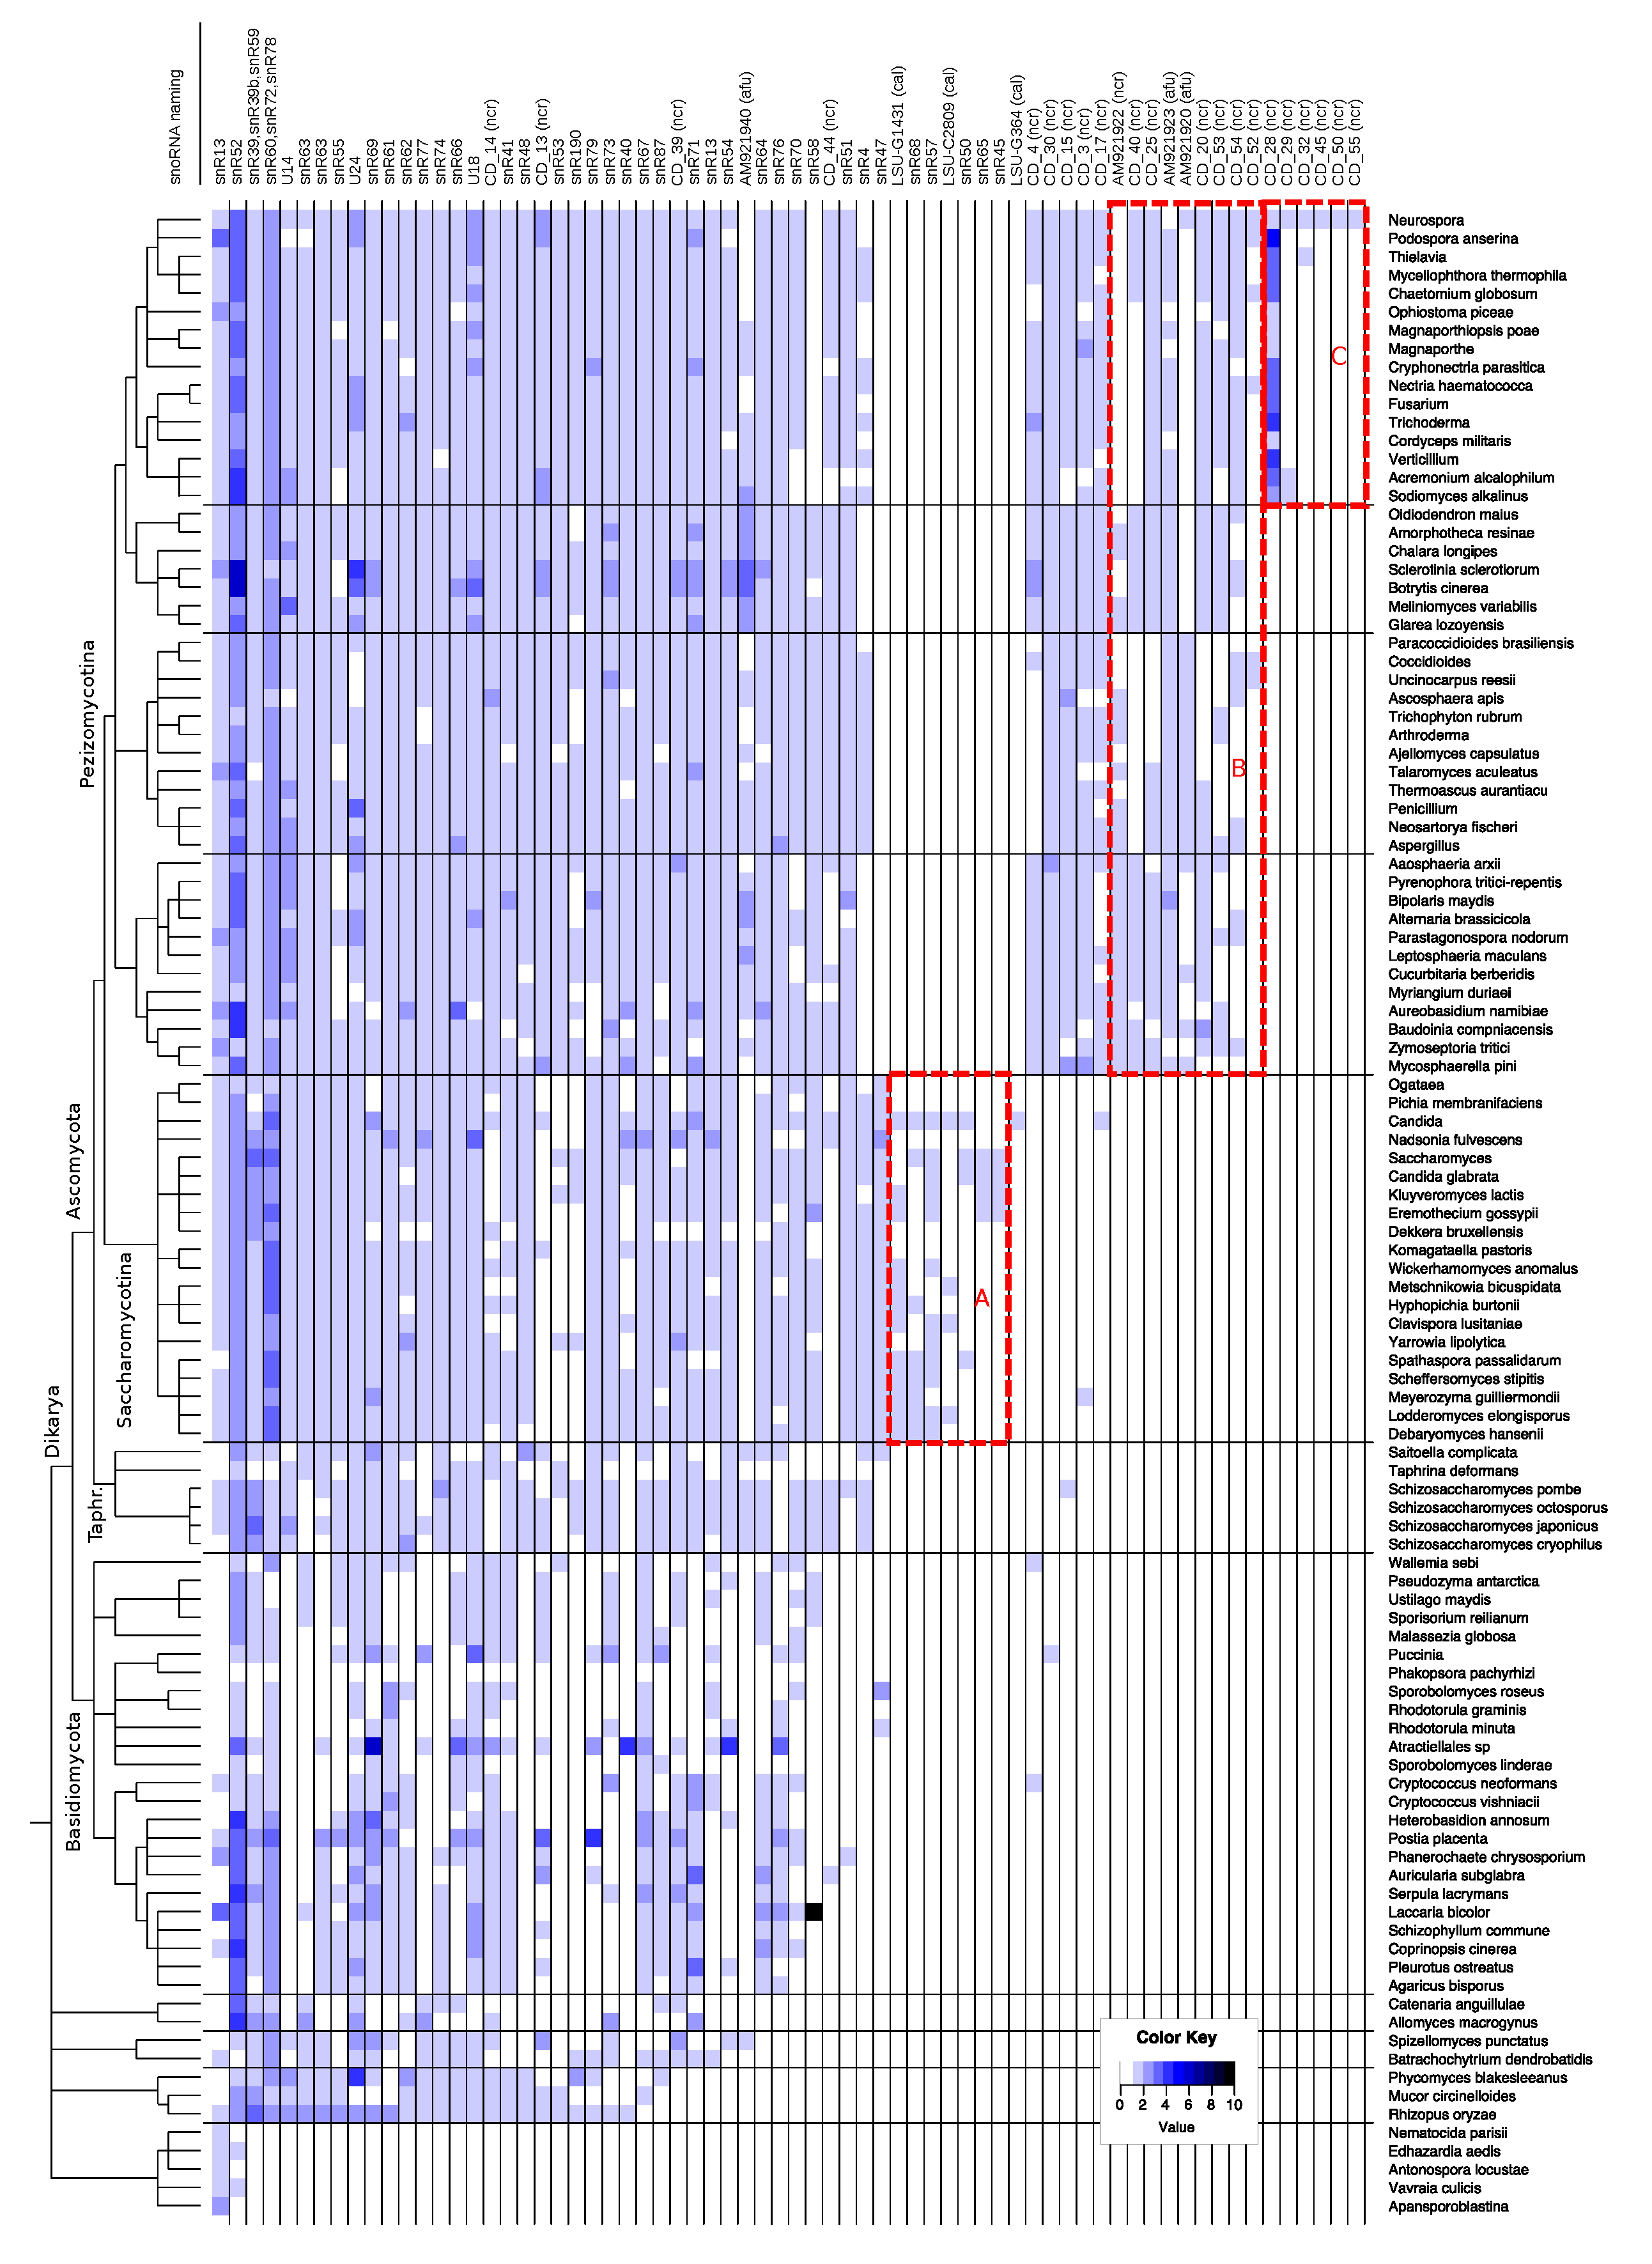
\includegraphics[width=1.05\textwidth]{pics/CD_snoRNAs_collapsed.short_naming.eps}
  \caption{A heatmap of
    \snostrip-detected \cd s is shown on the previous site. Each column represents a specific \sno\
    family, while each row either represents a certain species or
    genus. A taxonomic classification is shown on the left hand side. The amount of
    \sno s detected in a specific species and \sno\ family is encoded in a
    blue color scheme. Lineage specific families are boxed (A:
    Saccharomycotina, B: Pezizomycotina, C: Sordariomycetes). %Single
%    \sno\ detections in lineages without any other predictions are either marked with 'X',
 %   '$\star$', or '!', depending on their family-specific functionality. For further details see text.
  }
  \label{fig:heatmap_CD_snoRNAs} 
\end{figure*}



Almost half of all \cd\
families are traceable down to the root of fungi (32/68), i.e., at least one early
branching fungal lineage is attested to carry this \sno\
family, such as Microsporidia, Mucoromycotina, Chytridiomycota, or
Blastocladiomycota. Additionally, several families are found to be
lineage-specific, e.g., seven in Saccharomycotina (see box 'A' in
Figure \ref{fig:heatmap_CD_snoRNAs}), nine in Peiziomycotina (box
'B'), and six in Sordariomycetes (box 'C'). These lineages map exactly to the
clades where original \sno\ data originated from.


In contrast to lineage-specific families, lineage-specific losses of
\sno s are also detectable. Basidiomycota, for example, are not found
to contain orthologs of families snR48 (CD\_8), snR190 (CD\_16), or U14 (CD\_37), while in
Saccharomycotina, no trace is found of \sno s of family AM921940
(CD\_41). Members of Nc\_CD\_40 (CD\_40) are not detected in Eurotiomycetes, while
Sordariomycetes are attested to miss homologs of families snR39/b (CD\_47) and
snR58 (CD\_68). In some other cases, one or two representatives are found in
lineages where the remaining species do not contain this particular
family. In these lineages, only the analysis of target interaction
might answer the question whether this single \sno\ is a true member
of the family or merely an artifact.


%\mysubsection{Box H/ACA \sno\ Families}
%
%\begin{figure}
%  \centering
%  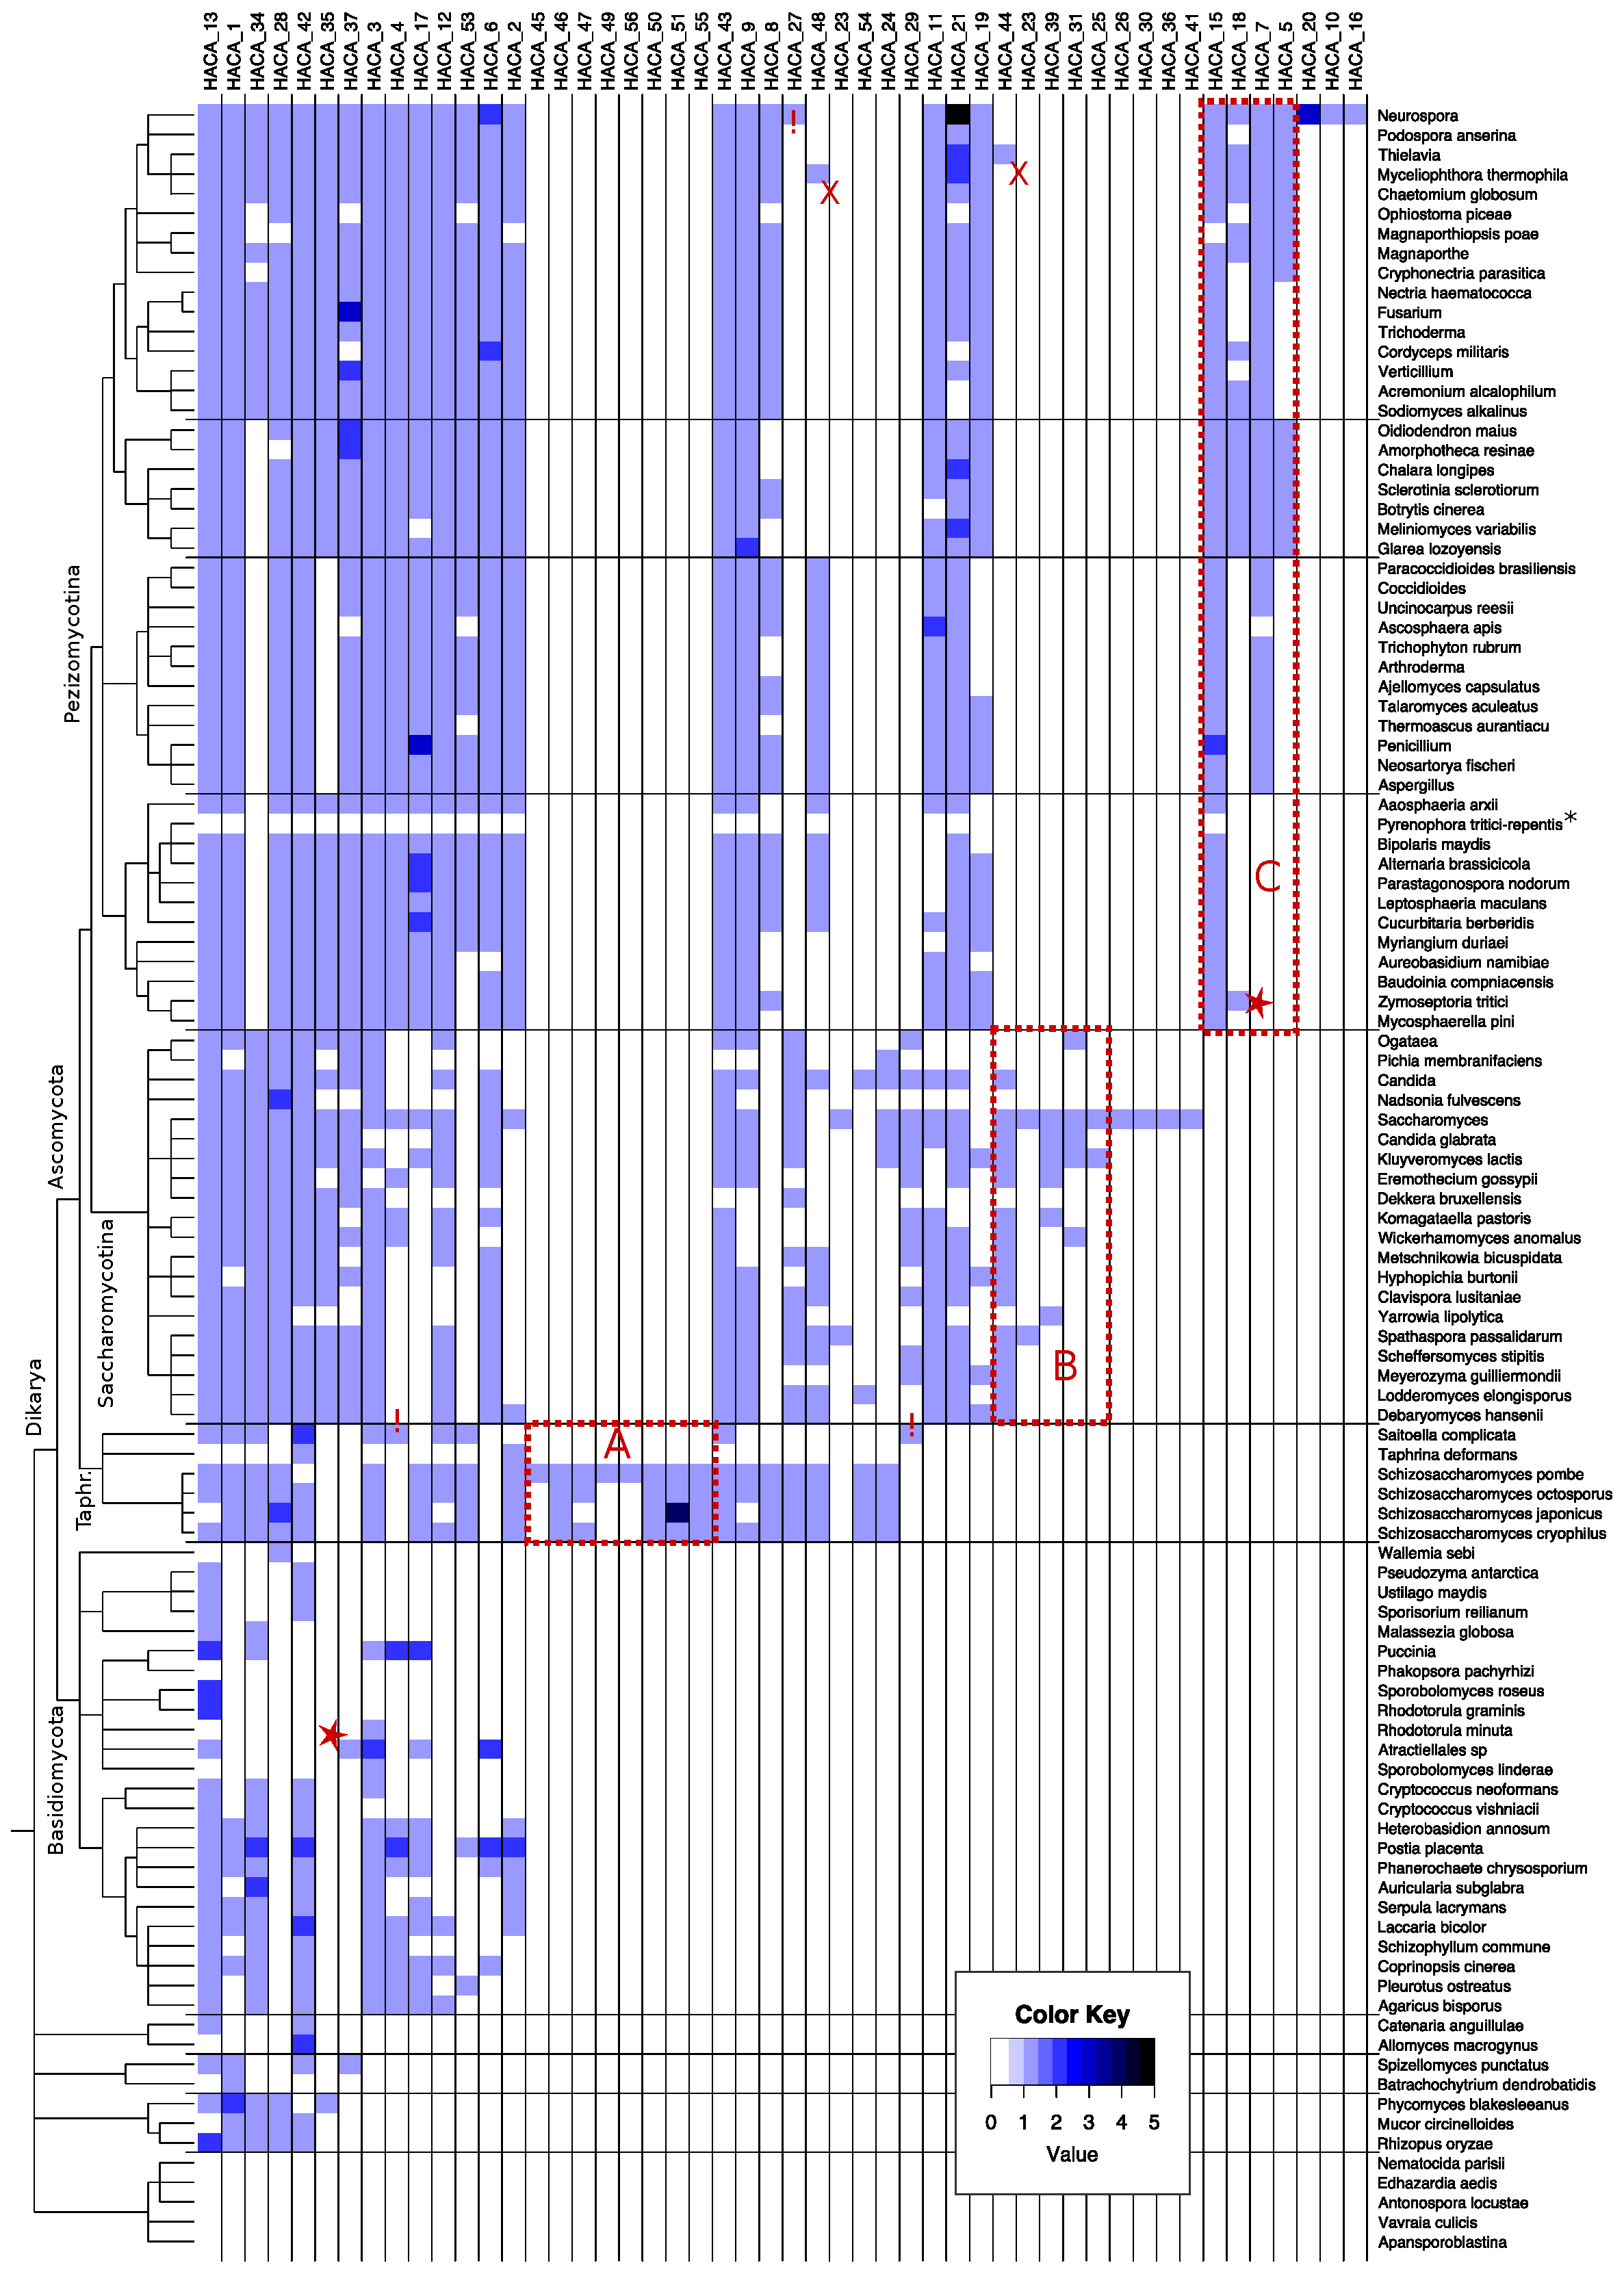
\includegraphics[width=\textwidth]{PICS/FUNGI/HACA_snoRNAs_collapsed.eps}
%    \caption{A heatmap of
%    \snostrip-detected \haca s is shown on the previous site. Each column represent a specific \sno\
%    family, while each row either represent a certain species or
%    genus. A taxonomic classification is shown on the left side. The amount of
%    \sno s detected in a specific species and \sno\ family is encoded in a
%    blue color scheme. Lineage specific families are boxed (A:
%    Schizosaccharomycotina, B: Saccharomycotina, C: Pezizomycotina). Single
%    \sno\ detections in lineages without any other predictions are either marked with 'X',
%    'star', or '!', depending on their family-specific functionality. For further details see text.}
%  \label{fig:heatmap_HACA_snoRNAs}  
%\end{figure*}

Compared to \cd s, only seven \haca\ families (out of 50) are detected in early branching fungi
and Dikarya. None of these is detected in Microsporidia
leaving this clade completely without any annotated \sno\ candidate. It
is apparent, however, that \haca s shows substantially
more lineage specific innovation and deletion events than observed in \cd s, see supplementary Figure S5.

%In total, seven families are exclusively found in Schizosaccharomyces
%(red box 'A' in Figure \ref{fig:heatmap_HACA_snoRNAs}),
%five in Saccharomycotina (red box 'B'), four in Saccharomyces, four in
%Pezizomycotina (red box 'C'), and two are exclusively present in Neurospora. 
In total, 22 out of 50 H/ACA families are merely found in a
small subset of species. Moreover, several families are found in two
or more lineages but seem to be completely lost in others, such as snR42 (HACA\_33),
AJ632014 (HACA\_56), and snR33 (HACA\_24). They are present in Taphrinomycotina and
Saccharomycotina but cannot be found in Pezizomycotina. 
%In other families it
%occurs that just a single \sno\ molecule is detected amongst all organisms
%of a particular lineage raising the question whether this sequence is
%indeed functional or the remains of the vanished \sno\ gene. Several
%such cases are marked in Figure \ref{fig:heatmap_HACA_snoRNAs}. Furthermore, their target binding ability is classified to better capture the
%implication made by these single \sno: Categories are 'non-functional'
%(red 'X'), i.e., the \sno\ is not predicted to bind the conserved and annotated
%target, 'marginal functional' (red '$\star$'), meaning that the predicted
%mfe is above -30 kcal/mol, or 'highly  functional' (red '!') stating
%that the family specific target region can be bound extraordinary
%well. In seven detected cases, two are found to be non-functional, two
%are found to be functional with a minimum free interaction energy
%above -30 kcal/mol, while the remaining three sequences are predicted to bind
%the target region exceptionally.


\begin{figure*}
  \centering
  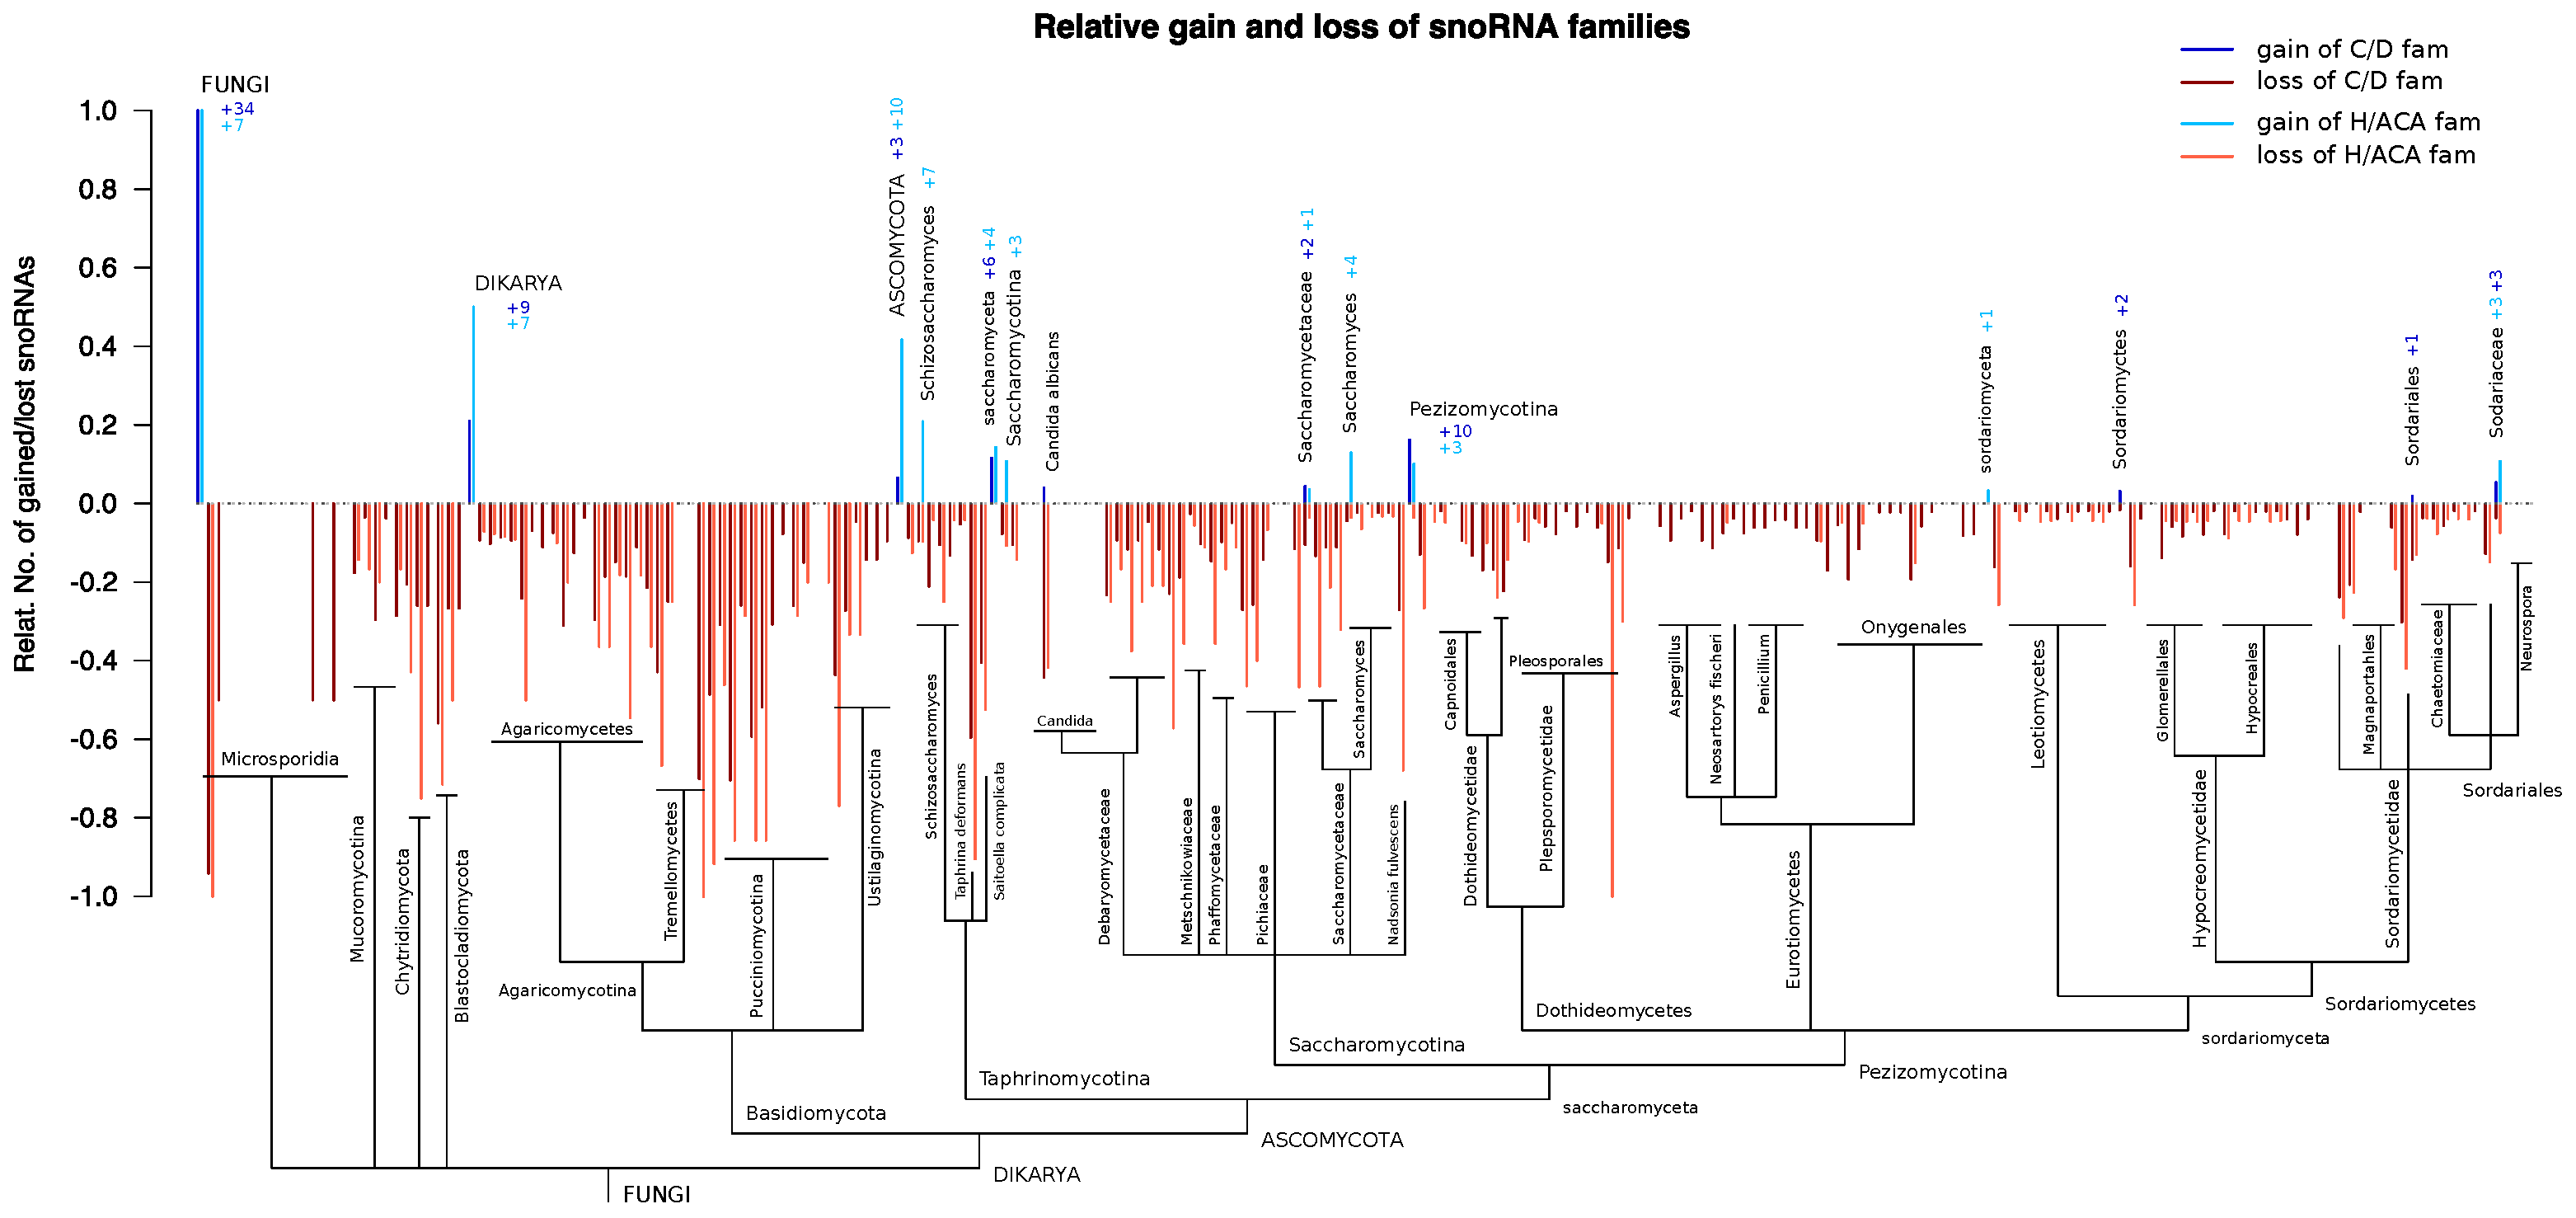
\includegraphics[width=\textwidth]{pics/fungi_relative_gain_loss.eps}
  \caption{Relative number of gains and losses of entire snoRNA families during fungal
evolution. The relative gain is the number of gained snoRNA families compared to the
observed number of snoRNA families. The relative loss describes the number of lost
snoRNA families compared to the number of snoRNA families in the parent node of the
phylogenetic tree.}
\label{fig:relative_innovation_deletion_event}
\end{figure*}


Another noticeable observation is that not a single \haca\ is
found in \Ptt\ (marked with an asterisk in the supplement Figure). This stands in sharp contrast to C/D \sno\ sequence,
where \ptt\ orthologs are found in nearly all families that are
present in the \ptt-containing Dothideomycetes lineage.


\paragraph{\textbf{Evolutionary event in snoRNA history}}

With the help of the \epope\ software, we identified the last common ancestor of each individual snoRNA family and found the most parsimonious estimate for the number of paralogs at the inner nodes of the tree. 
We deduced gain and loss event of individual paralogs of each snoRNA family and summarized this information for all analysed snoRNA families to retrieve a full picture of the evolution of  snoRNAs in fungi.

Relative innovation and deletion events mapped to the pre-ordered
nodes of the NCBI-derived taxonomic tree up to species level are shown in
Figure \ref{fig:relative_innovation_deletion_event}, see supplementary Figure S6 for a version with absolute values.
We observe a large amount of \sno\ families that emerged at each
major branch point along the backbone of the taxonomic
tree. A total of 34 \cd\ families could be traced to the root of
fungi, indicating an even more ancient origin. At the root of 
Dikarya, Ascomycota, Saccharomyceta, and Pezizomycotina, a total
 of 9, 3, 6, and 10 families arose, respectively. A similar picture is drawn in
case of \haca s where 7 families could be traced to the root of
fungi and additional 7, 10, 4, and 3 families are gained at the root
of Dikarya, Ascomycota, Saccharomyceta, and Pezizomycotina. 
According to our methods, we could only detect innovations of snoRNA families at branches leading to the five starting species.  

Microsporidia seem to have lost almost the entire snoRNA complement that has been present before their split during the evolution. 
Only two \cd\ families seem to be conserved in this lineage. 
Gardner \emph{et.~al} formerly mentioned the remarkable absence of \sno\ genes in this clade, although all components of the \sno\ machinery are clearly present
\cite{Gardner:2010}. 
We agree with these researchers that without further experimental investigations in these fungi we cannot state a true loss or a rearrangement of their snoRNA repertoire. 

%On the
%contrary, losses of seven or more families at a particular point in
%the tree, have only a little relative effect when a large fraction of
%\sno\ families has been gained before, cf. losses of Dothideomycetes
%(-8 C/D, -8 H/ACA) and Eurotiomycetes (-7 C/D, -10 H/ACA) in the
%Figure \ref{fig:relative_innovation_deletion_events}. 

When focusing on species level, it is frequently observed that single
organisms seem to have lost a large amount of their snoRNAs, i.e. in the  Basidiomycota lineage. 
Especially \wse\ and several Pucciniomycota seem to have lost nearly their entire set of \haca s (\wse: 92\%, \rmi: 86\%,
or \sli: 86\%). The impact on \cd s is more moderate (0.26 on
average). A potential correlation with significantly smaller genome
sizes in Pucciniomycota was not detected (data not shown). The
previously mentioned loss of the entire \haca\ set in \Ptt\ is also clearly
visible. Other organisms such
as \pan\ and  \opi\ also show an increased loss rate (\pan: 15\% C/D
and 13\% H/ACA; \opi: 30\% C/D and 42\% H/ACA). 


%\begin{figure}
%  \centering
%  \includegraphics[width=0.95\textwidth]{PICS/FUNGI/taxonomic_tree_ncbi_collapsed.eps}
%  \caption[Innovation and Deletion events in fungal \sno\
%  history.]{Innovation and deletion events in fungal \sno\ evolution.}
%\label{fig:absolute_innovation_deletion_events}
%\end{figure}

\paragraph{\textbf{Novel \emph{Candida albicans} \sno s are lineage-specific}}

%To investigate the fate of intron encoded ncRNAs in species that
%suffered massive intron loss, Mitrovich \emph{et.~al} identified novel \sno\ sequences in different
%species including \calb\ based on \emph{de novo} prediction and
%expression values \cite{Mitrovich:2010}. For \calb, 40 potential \cd\
%sequences were annotated and 36 of them showed high sequence similarity
%to known budding yeast \snos. One of the remaining sequences shares a homologous target
%binding region with a known \ncr\ \sno\ (CD\_39), while the other three
%candidates combine no obvious homology to already published \snos. 
%
%Family CD\_69 (LSU-C2809 in \cite{Mitrovich:2010}) is found in all other \emph{Candida} organisms and two additional
%Saccharomycotina. The initially predicted
%target interaction with 25S-4055 (\calb: 25S-3118) is also highly
%conserved across all identified \snos\ (ICI score: 1.813).
%Homologs of the \calb\ sequence CD\_71 (LSU-G1431) were successfully
%traced in most Saccharomycotina, except for Saccharomycetaceae. The
%extraordinary ICI score of 1.289 indicates a highly conserved target
%binding capability with position 25S-2490 (\calb: 25S-1740).
%The third novel \sno\ candidate CD\_72 (LSU-G364) was merely detectable in two closely related
%species, \cdu\ and \ctr, respectively. Although all three sequences
%show a highly conserved target region upstream of box D, it is not
%possible to reliably identify a conserved target interaction based on
%such a small set of closely related organisms. 
%%This is due to conserved \snos\
%%on the one hand and, obviously, highly conserved target RNAs on the
%%other hand. This makes each predicted interaction that is traceable in
%%a single organisms
%% also traceable in the other species. In case of this particular
%% family, 
%Six potential target
%interactions have an ICI score above 0.9 although their mean minimum
%free binding energy is relatively high (between -7.3 and -9.0).
%
%%Please note that the originally denoted modification sites are
%%not equal to the \calb\ specific modification sites published here since
%%different 25S rRNA sequences have been used. The authors named their
%%novel identified sequences with respect to their target predictions
%%but die not provide the corresponding targetRNA sequences. 
%


Mitrovich \emph{et.~al} identified four novel \sno\ candidates among their set fo 40 \sno\ genes that showed no high sequence similiarity towards already annotated budding yeast sequences \cite{Mitrovich:2010}. One of these sequences is found to share a homologous target
binding region with a known \ncr\ \sno\ (Nc\_CD\_39). Families LSU-C2809 and LSU-G1431 in \cite{Mitrovich:2010} (\snostrip: CD\_69 and CD\_71)  are exclusively present in Saccharomycotina except for Saccharomycetaceae. They are also found to share an extraordinary conserved target-interaction with ICI scores of 1.813 (25S-4055; \calb:~25S-3118) and 1.289 (25S-2490; \calb:~25S-1740), respectively. The remaining family LSU-G364 (CD\_72) is merely found in two closely related species: \cdu\ and \ctr.



\paragraph{\textbf{Fission Yeast Specific \sno s}}

%Similar to \calb, several \sno s published in the fission
%yeast \cite{Li:2005} are found to be lineage or even species
%specific. HACA\_46 (AJ632008 in \cite{Li:2005}) is annotated to be a double guiding \sno\ and shows
%indeed two conserved pseudouridylation pockets in both hairpins across
%the four members of Schizosaccharomyces. The predicted modification
%site for hairpin 1 (HP1) is also known to be modified in \sce\ (25S-2314) and
%human. The correspondung budding yeast family HACA\_36 (snR86),  
%which is experimentally confirmed to guide
%pseudouridylation at this precise position, is merely a functional
%homolog to the Schizosaccharomyces specific HACA\_46 \sno\ since
%the functional target binding site resides in hairpin 2 (HP2) instead of the first
%hairpin. A similar situation is found in HACA\_47 that shares a
%conserved and annotated HP2 target (25S-2060). This position is again
%known to be modified in both budding yeast and human. But although both
%anti sense elements (ASE) are located in hairpin two in \spo\ and \sce\, sequences of both
%groups share far too little sequence similarity to be denoted as homologous
%families on sequence level. However, they are clearly functional homologs. 
%
%While families HACA\_50 and HACA\_55 are present in all
%Schizosaccharomyces species the true modification site remains
%secret. The putative target in  \sno\ HACA\_50 was neither
%found to be conserved in other Schizosaccharomyces and
%conserved predictions for the orphan target sites in HACA\_55 have not
%been detected by \snostrip.  
%
%The three sequences HACA\_45, HACA\_49, and HACA\_56 are exclusively
%found in \spo. The correct assignment of a functional modification
%site is nearly impossible for single sequences, and hence these
%originally orphan guides remain orphan.
%
Similar to \calb, several \sno s published in the fission
yeast \cite{Li:2005} are found to be lineage or even species
specific. In the original publication, 12 sequences have not been mapped to budding yeast \sno s and 7 of them have no predicted target interaction. By means of \snostrip, AJ632008 in \cite{Li:2005} (HACA\_46) and AJ632011 (HACA\_47) have been detected to be functional homologs to snR86 (HACA\_36) and snR5 (HACA\_27), respectively. The first one includes a switch from a HP1 target in \spo\ to a HP2 target in \sce, while the latter two families share far too little sequence similarity to be denoted as homologous sequences. Families AJ632018 (HACA\_9), AJ632010 (HACA\_48), AJ632016 (HACA\_53), and AJ632012 (HACA\_54) are found to be conserved outside of Taphrinomycotina. The first two families map to families with an annotated target while the latter families lack such a finding. The remaining sequences are either specifically detected in Schizosaccharomyces (AJ632009 (HACA\_50), AJ632017 (HACA\_51) and AJ632013 (HACA\_55)) or exclusively found in \spo\ (AJ632015 (HACA\_45), AJ632019 (HACA\_49), and(AJ632014 (HACA\_56)).


%\TODO{
%What happened to  AJ632018?? mapped to HACA\_52, but lost somehow...
%Mapped to HACA\_9, but mapping was lost...
%\Spo\ sequences that were not mapped originally to already annotated budding yeast sequences: AJ632008 - AJ632019. AJ632008-AJ632012 have predicted, annotated target interactions. the remaining families are denoted as orphan.
%
%HACA\_46 (AJ632008) and HACA\_47 (AJ632011) are functional homologs to budding yeast annotated sequences. 
%
%
%HACA\_50 (AJ632009), HACA\_51 (AJ632017) and HACA\_55 (AJ632013) are found in all Schizosaccharomyces, but lack confident prediction of target interaction. 
%Sequences HACA\_45 (AJ632015), HACA\_49 (AJ632019), and HACA\_56 (AJ632014) are exclusively found in \spo. 
%
%Conserved outside of Taphrinomycotina with an annotated target: HACA\_48 (AJ632010), HACA\_9 (AJ632018).
%conserved outside of Taphrinomycotina with unannotated target prediction: HACA\_53 (AJ632016), HACA\_54 (AJ632012)
%
%What about the remaining 5 snoRNA candidates - HACA\_48 (AJ632010), HACA\_51 (AJ632017), HACA\_9 (AJ632018), HACA\_53 (AJ632016), and HACA\_54 (AJ632012)?
%
%% HACA\_48 conserved in Taprhino, Saccharom, Dothideom, Eurotiom. ICI: 1.15 annotated
%% HACA\_51 conserved in Taphrino, 18S-400 in two of four organisms, ICI: 0.48 HP2
%% HACA\_9 conserved in Ascomytcota, HP1 target: 25S-1962, ICI 1.17 HP1, annotated target
%% HACA\_53 conserved in Taphrino, Pezizomycotina, potential target 18S-1302, ICI 0.82, not annotated
%% HACA\_54 conserved in Taphrino, candida, debaryomyces, potential targte found: 25S-3439, ICI 1.22
%
%
%
%}



\subsection{Conservation of Target Interaction}

In accordance to their conserved function, each
\sno\ family can either be classified as single guide, double guide,
or orphan \sno. Single guide sequences share a conserved and
functional anti sense element either upstream of box D or D' in \cd\
or either in hairpin 1 (HP1) or hairpin 2 (HP2) in \haca s. Double
guide \sno s exhibit functional target binding
regions in both positions. Orphan \sno s have no known and conserved
target interaction. Normally, each individual \sno\ is predicted to be capable of binding
several regions of different targetRNAs. But target predictions that
are based on single sequence predictions
are not overly convincing in a biological point of view. 

\begin{figure*}
  \centering
  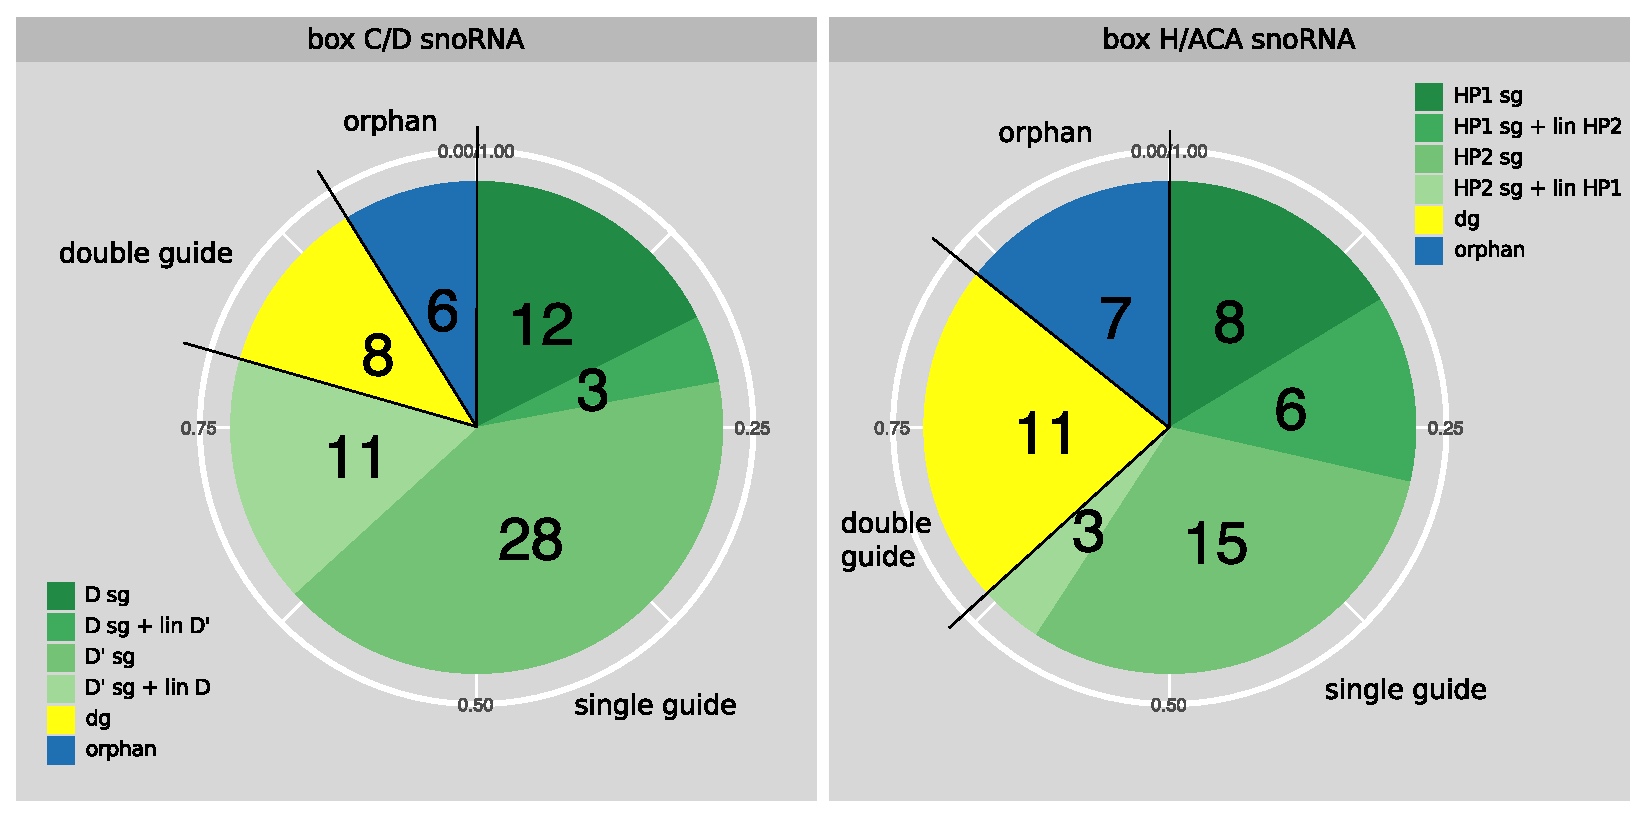
\includegraphics[width=0.9\textwidth]{pics/pieCharts_snoRNAs_modified.eps}
  \caption[Classification of \sno\ families as single or double guides.]{Pie
    chart of both major \sno\ classes. A \sno\ family is classified based on
    its conserved target prediction either as single guide (sg), single
    guide with a lineage specific target in its non-conserved target
    region (lin),
    double guide (dg), or orphan.}
  \label{fig:pie_charts}
\end{figure*}

Within the 68 \cd\ families, the large majority (40) is found to be
\textit{true} single guides. 28 families share a functional D' target
and the remaining 12 families a conserved D box associated binding
site. An additional amount of 14 \cd\ families are \textit{predominantly}
found to be single guides, i.e., these families share exactly one highly
conserved target binding region (three families share a conserved D target
while 11 families share a functional D' target), whereas the other
target region is only found to be functional in subset of
organisms. Eight families harbor two
functional target binding regions that are conserved throughout all
lineages where these families are detected. 
Six families
 are originally denoted as orphan \sno\ meaning that no potential interaction has been
 published thus far. In case of \haca s, 23 families are \textit{true}
 single guides: 8 families share a conserved pseudouridylation pocket
 in hairpin 1 and 15 families share a HP2 target. Further 6 families
 comprise a lineage specific HP2 target besides their overly
 conserved target in hairpin1. The opposite situation can be seen in 3
 \haca\ families. 11 families are found to be double guides, while 7
 families are orphan. A summary of the \sno\ classification can be seen
 in Figure \ref{fig:pie_charts}.  Detailed information about each family and the
 \snostrip-assigned target interactions, e.g., alignment position of
 the modification site, ICI scores, and mean minimum free energy
 values, can be found in the supplement. 


%%%%%
%% DOUBLE GUIDE SNORNAS
%%%%%
Solely a minority of \cd s is found to contain two overly
conserved target regions upstream of box D and D'. However, except for '\sno\ clans'
CD\_5 and CD\_19, none of
the remaining six families is traceable amongst all major fungal
lineages. Two families, Nc\_CD\_17 (CD\_17) and  AM921920 (CD\_35), are found in Pezizomycotina
while snR47 (CD\_67) is exclusively found in Saccharomycotina. The remaining
families are either found in Sordariales Nc\_CD\_32 (CD\_32), a subgroup of
Sordariomycetes, or in Glomerellales and Neurospora Nc\_CD\_29 (CD\_29). 

Double guide \haca\ families occur more frequent. 11 families are originally annotated as
double guides and most of their targets are convincingly confirmed
by \snostrip. Furthermore, double guided \haca s are commonly traceable across a wide
range of fungal organism. Four families have their origin at the root of Dikarya or
even further back: Nc\_HACA\_2 (HACA\_2), snR3 (HACA\_3), snR8 (HACA\_6), snR80 (HACA\_37). Two more families are traced to the root of
Ascomycota: snR5 (HACA\_27), snR49 (HACA\_29), whereas the remaining five families are lineage-specific (two
found in Saccharomycotina, snR82 (HACA\_31), snR161 (HACA\_39)) or genus-specific (two found in
Saccharomyces, snR81 (HACA\_26), snR83 (HACA\_30); one found in Schizosaccharomyces,  AJ632008 (HACA\_46)).

Family snR3 is published to guide three targets in both the budding yeast
and fission yeast (annotated as AJ632000 in \spo, HACA\_3 in \snostrip); HP1 is known to guide modification at position 25S-3311 (25S-2129 and
25S-2216 in the budding and fission yeast, respectively), while there
are two targets in HP2; 25S-3449 and 25S-3315 (\sce\ 25S-2264 and
25S-2133, \spo\ 25S-2351 and 25S-2220). All three targets are found to
be conserved across Dikarya. In the original Neurospora publication,
however, HP1 is annotated to guide the isomerization at position
25S-1200 (25S-401 in \Ncr). This guiding capability is not found to be
conserved throughout the members of this family unlike the yeast
annotated target which is also convincingly predicted in Neurospora
species, even with a lower interaction energy. 

\paragraph{\textbf{Orphan \sno}}
Orphan \sno s are sequences without a known target interaction on both
potential anti sense elements. In the originally published \sno\ datasets of five different fungi, orphan \cd s were annotated for \sce\
(2 sequences), \ncr\ (2), and \afu\ (9). In addition to these sequences,
11 \ncr\ \sno s have been published with predicted targets
based on single sequence target prediction only. Since there is
usually more than just one valuable prediction for a single \sno, these predictions might be
misleading until they are evaluated under the light of
evolutionary conservation or the original \sno\ sequences are mapped to species with verified
targets.

A detailed summary of these sequences and their predicted targets with
respect to evolutionary conservation is shown in supplementary Table S12. Highly conserved
target interaction that are predicted by \snostrip\ are shown in Table \ref{tab:orphan_cd_snoRNAs_short}. 

\begin{table}
  \caption{Assigning putative targets to previously
    orphan \cd s. Families that do not contain sequences with
    experimentally verified targets are marked with '*'. }
  \label{tab:orphan_cd_snoRNAs_short}
  \begin{center}
    \begin{footnotesize}
      \begin{tabular}{c|c|c|c|c}
      original&&target&&snostrip\\
      name&\raisebox{1.5ex}[-1.5ex]{box}&position&\raisebox{1.5ex}[-1.5ex]{ICI
      score}&name\\
  \hline
  Nc CD\_10&D'&18S-479&1.13&CD\_10\\
\hline
  Nc CD\_26&D'&25S-3836&0.86&CD\_26\\
\hline
  Nc CD\_53&D'&25S-3500&0.71&CD\_53*\\
\hline
  Nc CD\_54&D'&U60-70&1.43&CD\_54*\\
 \hline
  AM921936&D'&25S-4198&1.50&CD\_36\\
\hline
  AM921937&D'&18S-479&1.13&CD\_31\\
\hline
  AM921938&D'&25S-3474&1.19&CD\_7\\
\hline
  AM921939&D'&18S-179&1.09&CD\_15*\\
\hline
  AM921940&D&18S-849&1.21&CD\_41*\\
\hline
  AM921941&D'&18S-630&1.36&CD\_24\\
\hline
  AM921942&D&18S-456&1.71&CD\_37\\
\hline
  AM921944&D'&18S-1083&1.57&CD\_49\\
\hline
  AM921945&D'&25S-3836&0.86&CD\_26\\

    \end{tabular}
    \end{footnotesize}
  \end{center} 
\end{table}

Unfortunately, potential targets for both orphan \ncr\ \sno s are not
unambiguously discovered by \snostrip. The best prediction yields an
ICI$_{sno}$ score of 0.71 for family Nc\_CD\_53 (CD\_53) and is loosely found in
several Pezizomycotina species (25S-3500, mean mfe: -11.56). The
second family Nc\_CD\_55 (CD\_55) is exclusively found in Neurospora preventing a
functional analysis of potential targets based on conservation aspects. 

In case of both budding yeast \sno s (snR4, snR45), no potential target is found
across canonical target sequences, although family snR4 is found to be
present in several fungal lineages such as Taphrinomycotina,
Saccharomycotina, and several Pezizomycotina species. Family snR45, on
the other side, is exclusively found in Saccharomycetaceae.

The picture looks much better in case of \afu\ orphan \sno s. The
\snostrip\ pipeline was able to map seven out of nine orphan \cd s
to families with experimentally validated targets. These target
interactions are also predicted in \afu. Both remaining families
(marked with '*' in Table \ref{tab:orphan_cd_snoRNAs_short}) are
traceable in the majority of Pezizomycotina species and putative
target sites are also conserved making the \snostrip\ results
plausible despite a missing experimental verification.

The set of 11 \ncr\ \sno s, with predicted targets but without homologous
relations to other known \sno s,
comprised 16 distinct targets published in the original publication \cite{Li:2005}.
Ten of these targets were confirmed through a conserved prediction using \snostrip.
Three targets were annotated as tRNA modification
sites and hence, are not checked in this study. However, these target
regions show no conserved and obvious base pairing capabilities to
canonical target RNAs such as rRNAs or snRNAs. The remaining three
target sites were predicted based on falsely detected D' box
motifs and thus, are neither biologically correct nor conserved across
species. In two cases, evolutionary conserved box motifs are
identified and convincing target sites are predicted by \snostrip\
(Nc\_CD\_10, D' target, ICI: 1.13; Nc\_CD\_26, D' target, ICI: 0.86), see Table
\ref{tab:orphan_cd_snoRNAs_short}.

Family NC\_CD\_54 (CD\_54) was originally published to guide modification at
25S-1648 (\ncr\ 25S-667; D target) \cite{Liu:2009}. By means of
\snostrip, family Nc\_CD\_54 is detected amongst all Pezizomycotina lineages and a
highly conserved target region is clearly
visible upstream of box D', originally denoted as orphan. This region shows convincing base pairing capabilities to
U6-70 (\ncr\ U6-55) in virtually all identified organisms. The high
ICI$_{sno}$ score of 1.43 and the low mean mfe of -18.10 kcal/mol
further promote the correctness of this prediction, see Table
\ref{tab:orphan_cd_snoRNAs_short}. The initially
annotated D target, on the other hand, is not found to be conserved outside of Neurospora.\\

\begin{table}
  \caption[Potential targets for orphan \haca s.]{Assigning putative targets to previously
    orphan \haca s. Families that do contain sequences with
    experimentally verified targets are marked with '*'. }
  \label{tab:orphan_hacas_short}
  \begin{center}
    \begin{footnotesize}
      \begin{tabular}{c|c|c|c|c}
        original&&target&&snostrip\\
        name&\raisebox{1.5ex}[-1.5ex]{box}&position&\raisebox{1.5ex}[-1.5ex]{ICI
            score}&name\\
        \hline
        Nc HACA\_7&HP2&25S-3500&1.26&HACA\_7\\
        AM921943&HP2&25S-3374&1.12&HACA\_21*\\
        AJ632012&HP2&25S-3439&1.22&HACA\_54\\
        AJ632016&HP2&18S-1302&0.82&HACA\_53\\
        AJ632018&HP1&25S-1962&1.17&HACA\_9*\\
      \end{tabular}
    \end{footnotesize}
  \end{center}
%  \vspace*{3mm}
\end{table}

Within the initial \haca\ datasets, orphan sequences were
published for \ncr\ (6 sequences), \afu\ (1), and \spo\ (8).
A detailed summary of these sequence can be seen in supplementary Table S17.

By means of \snostrip, eight orphan sequences are found to be conserved on sequence level and five of them include budding yeast sequences, providing experimentally validated target sites (Nc\_HACA\_11 matches
snR11, Nc\_HACA\_12 matches snR30, Nc\_HACA\_13 matches snR10, AM921943
matches snR32, and AJ632018 matches snR43). The three remaining \sno\
families comprise a 
conserved target in HP2, see Table \ref{tab:orphan_hacas_short}. Family Nc\_HACA\_7 is found to be a distant
homolog to family snR86 (HACA\_36) which is merely detected in Saccharomycetes
organisms. Nonetheless, both families are sufficiently predicted to
guide the validated isomerization of uridine at position
25S-3500. Due to large differences in sequence lengths (HACA\_36 is approx. 1kb long
; Nc\_HACA\_7 is $\sim$ 180nt in length), \snostrip\ was unable to detect a
potential common origin. Family AJ632012 (HACA\_54) is exclusively found in Schizosaccharomyces,
Candida, and Debaryomycetaceae. All species with a sufficient LSU sequence
are competently predicted to guide the pseudouridylation at position
25S-3439 (\sce 25S-2254). This position is not known to be modified
in the budding yeast, 
explaining the missing homologs in this clade. Family AJ632016 (HACA\_53), is
found across Taphrinomycotina and Pezizomycotina and is convincingly
predicted to accompany target binding at position 18S-1302. However, this position is not known to be modified in yeast or human by now.

Seven of 15 orphan \haca s are found to be conserved solely on genus or
species level, i.e., 2 orphan \ncr\ sequences are exclusively found in
the two other Neurospora organisms, while five \spo\ \sno s are either
found in all Schizosaccharomyces\ species (2) or in the fission yeast only
(3). Such a small set of species that share a homologous \sno\ sequence
makes an appropriate target prediction impossible. Hence, a sufficient
conclusion about their true function and, further on, about their
genuine existence in terms of a viable \sno\ molecule as well as its
biological necessity remains elusive.


\paragraph{\textbf{Lineage-specific Targets}}


Quite a few \cd\ families harbor a highly conserved target either at
their D or D' position. However, in a large amount of cases, it might
be that these families exhibit additional lineage specific target binding
capabilities on their 'non-functional' ASE. Such a functionality might
have evolved at a specific time point during evolution, and because of
a potential benefit, is retained in all of today's organisms descending
from this ancestor. 

\begin{figure*}
  \centering
  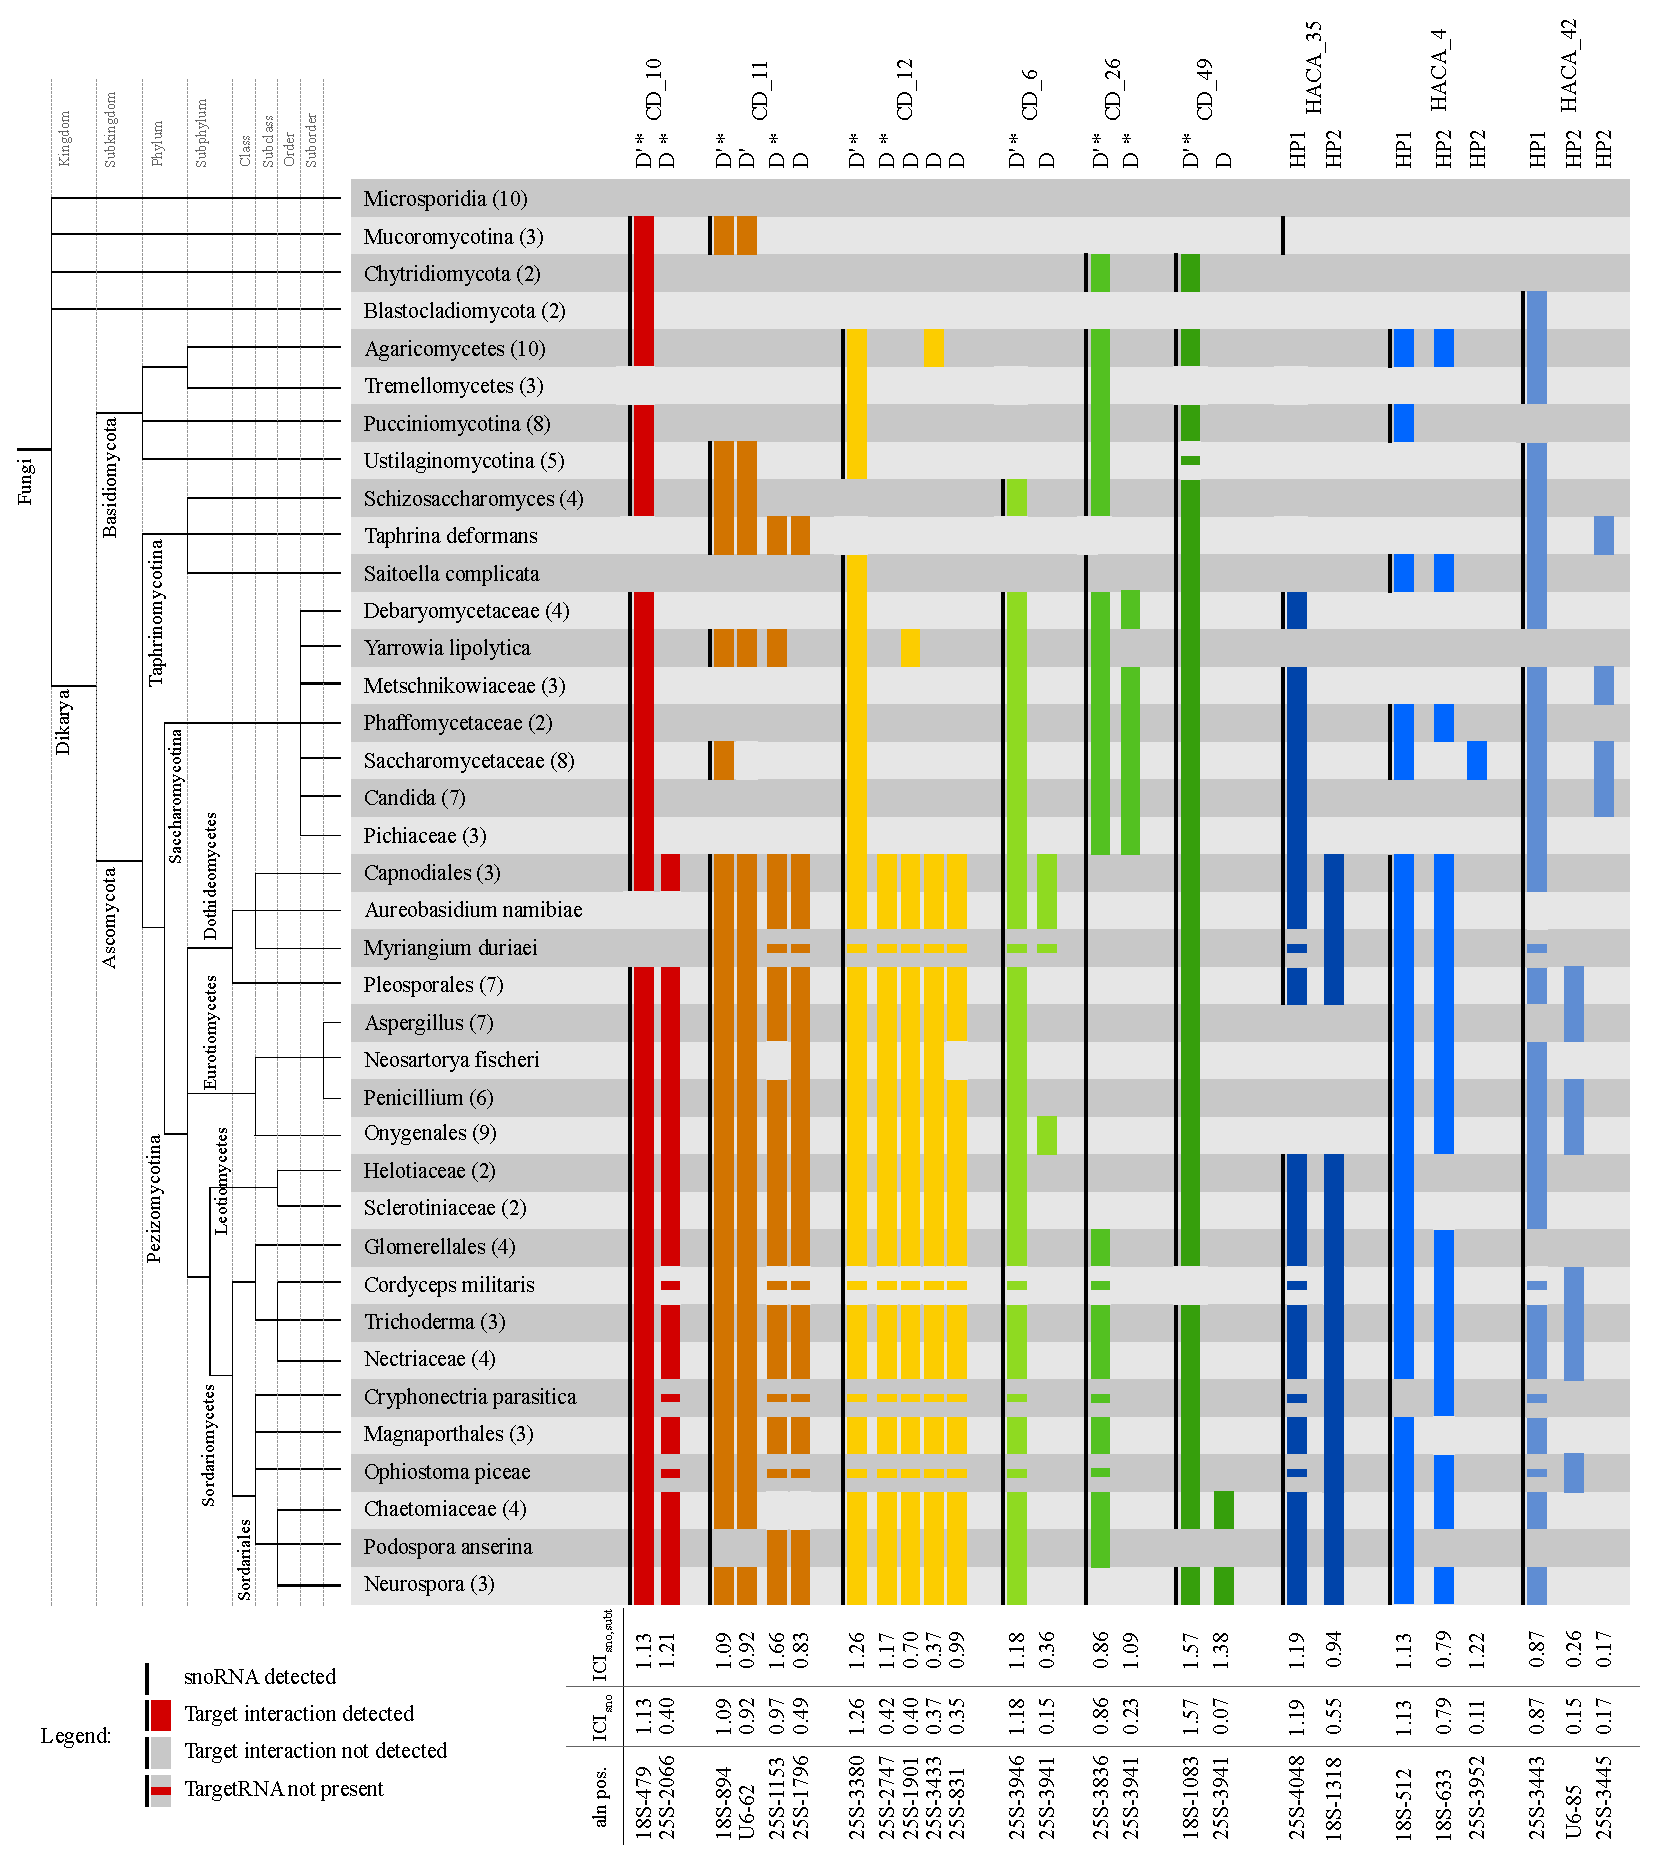
\includegraphics[width=\textwidth]{pics/conservation_lineage_specific_targets.eps}
  \caption{The conservation of predicted target interactions is shown for
    interesting single guide \cd\ families that exhibit an additional
    functional target at their 'non-functional' D box. Each family is
    depicted in a different color. The black bar in front of each
    family shows the presence of the family in a certain lineage or
    organism. The color bar shows that at least one target interaction
    was predicted in that lineage. The respective family name and target
    site can be seen on top while the alignment position and the
    corresponding ICI score are shown at the bottom. Experimentally
    confirmed interactions are denoted with '*'.}
  \label{fig:additional_targets}
\end{figure*}

Interesting \cd\ families with a previously annotated functional D'
targets and lineage specific D targets can be seen in Figure
\ref{fig:additional_targets}. Detailed information about all \sno\
families with an additional, lineage specific target are found in supplement Table S9.

Family snR87 (CD\_10), for example, with its experimentally verified target 18S-479
(18S-436; D' target), is detected in all analyzed fungal
lineages except for Microsporidia. Besides the functional D' region,
all Pezizomycotina species, whose large subunit rRNA is available, are
also predicted to guide an additional target upstream of their D
box. The target 25S-2066 (\ncr\ 25S-1042) has an ICI$_{sno}$ score of
1.21 amongst members in the Pezizomycotina subtree. The mean mfe is -13.19 kcal/mol.
Family snR53 (CD\_11) was shown to guide the methylation at position 18S-894 
(18S-796; D' target) in the budding yeast. The \snostrip-analysis
confirmed the \sno\ and this specific target interaction in a wide
range of fungi. An additional D' target, U6-62 (\sce\ U6-45), was
originally published in \ncr\ \cite{Liu:2009} based on single sequence
prediction. This interaction is also convincingly 
confirmed by \snostrip\ in all \sno s that were previously found to guide the
18S-894 target, except for Saccharomycetaceae, see Figure
\ref{fig:additional_targets}. Position 45 in U6 snRNA was not found to
be modified in the budding yeast
\cite{Machnicka:2013, Massenet:1998}. Due to missing analyses, no such
statement can be made in most other
fungal species. Since the ICI score for the U6 target is only marginal
smaller than for the 18S target, 0.89 to 0.94, respectively, and the
mean mfe value is found to be -13.78 kcal/mol (18S-894: -17.34), it is
thoroughly possible that this \sno\ is capable of modifying both
targets. However, two additional targets can be found for
the ASE upstream of box D: 25S-1153 and 25S-1796 (\ncr\ 25S-359 and
25S-790). Both candidates are predicted throughout all Pezizomycotina
species and, surprisingly, \Tde, a relative to the fission yeast. The
first interaction is additionally found in \Yli, a close
relative to the budding yeast. Because of its extraordinary low mean
minimum free energy of -21.12 kcal/mol, this target is assigned a high
ICI value of 1.66. The second putative interaction has an ICI score of
0.83 and a mean mfe of -11.50.

A highly interesting modification site is 25S-3941 (\sce\ 25S-2724)
whose actual methylation and the guidance by snR67 (CD\_26) was experimentally shown
\cite{Lowe:1999}. The conserved interaction of this position is
traceable in at least three different families, each in another fungal
lineage. Family snR67 is present in all Dikarya lineages and Chytridiomycota and shares a conserved D' target 25S-3836 (\sce\ 25S-2619)
that is predictable in all Dikarya except for Dothideomycetes,
Eurotiomycetes, and Leotiomycetes (ICI: 0.86, mean mfe: -23.03
kcal/mol). The D target 25S-3941, on the other hand,
is solely found in Saccharomycotina (ICI: 1.09, mean mfe: -15.34). Family snR51 (CD\_6) is found to share this target as a conserved D box
interaction in Onygenales and in a part of Dothideomycetes (ICI: 0.36, mean mfe:
-15.46). In a third family, snR54 (CD\_49), the
modification at 25S-3941 is predicted in Sordariales (ICI: 1.38, mean
mfe: -14.14, D target).
%These scattered interaction might have two different
%explanations; the interaction was either a subject of different target
%switches or it was completely lost at some point in fungal
%evolution. The latter scenario might have caused severe effects in
%development or growth of certain species such that the interaction
%might be reinvented in different lineages. However, either way
%indicates an importance for this specific methylation. 

In similarity to the box C/D \sno\ class, several \haca s comprise a
functional and highly conserved target guiding region in one hairpin
and show lineage-specificity in the other, see Figure \ref{fig:additional_targets}. 
A detailed summary can be found in the
supplement, see Table S15. Some of these functions might already been annotated, 
especially in \sno\ sequences of the budding yeast, see families
snR189 (HACA\_4) and snR191 (HACA\_42) which are in fact officially denoted as double guides
in \sce.  HP1 is highly conserved in both families and the corresponding
target binding capability is at least present in Dikarya. In their second hairpin,
however, they developed two different guiding functions that are
predictable in separate lineages. Family snR189, for example, is known to
guide the pseudouridylation at 25S-3952 in Saccharomycetaceae while
outside of this clade the \sno\ is mostly predicted to guide modification
at 18S-633. In snR191, on the other hand, the separation of both
target guiding functions becomes even more conspicuous. The budding yeast
annotated modification site is predicted in Saccharomycotina and \Tde\
(25S-3445), whereas the position U6-85 is predicted in a wide range of
Pezizomycotina.

Family snR32 (HACA\_21) is
predicted to guide the modification at position 57 (\ncr\ 54, \sce\ 54) in the
5.8S rRNA with its first hairpin in a large amount of Pezizomycotina
species (ICI$_{sub}$ = 0.73). This particular modification is not present in budding yeast
5.8S molecules which undoubtedly explains the missing predictions in
this subtree. On the contrary, the corresponding human position is found to
be pseudouridylated raising the possibility for this predicted
interaction to be an authentic and biological correct modification.
Based on the ICI$_{sub}$ score, a potential, alternative target at
position 25S-2813 is convincingly predicted with 1.07 in 19 out of
27 Saccharomycetales organisms. Since experimental evidence for this
precise position is missing, the prediction remains hypothetical.

\paragraph{\textbf{Target switches}}
Occasionally during evolution, novel guiding interactions are acquired
or present ones are lost in different species or lineages. It is,
however, much more uncommon that some target interactions are
translocated from one snoRNA to another. Therein, the position of the ASE
within the snoRNA sequence, upstream of box D/D’ or in HP1/HP2, is mostly
preserved but it happens seldomly that this position is also
shifted. Two highly complex rearrangements have been autmatically
detected by \snostrip. Each of these two '\sno\ clans' comprise two,
three or even more \sno\ sequences in each organism with distinct
target interactions. Due to target switches during fungal evolution,
these previously independent \sno\ sequences became connected. Table
\ref{tab:sno_clans} summarizes the target interactions that are convincingly predicted in the \sno\ clans CD\_5 (containing budding yeast sequences snR60, snR72, and snR78) and CD\_19 (snR52, snR56).
\begin{table}
  \caption{Interaction properties of four LSU modifications of CD\_5
    are shown. Properties for three SSU and two LSU methylations are
    given for clan CD\_19.}
  \label{tab:sno_clans}
\begin{center}
  \begin{scriptsize}
  \begin{tabular}{c|c|c|c|c}
    &&&&detected\\
    & \raisebox{1.5ex}[1.5ex]{modification}& \raisebox{1.5ex}[1.5ex]{ICI$_{sno}$}& \raisebox{1.5ex}[1.5ex]{$\varnothing$ mfe}&interactions\\
  \hline
  &25S-1806&0.79&-16.46&23.08\%\\
  &25S-1866&0.90&-19.49&24.61\%\\
  \raisebox{1ex}[3ex]{\rotatebox{90}{CD\_5}}&25S-1898&1.20&-25.80&25.38\%\\
  &25S-3615&1.00&-18.48&25.77\%\\
  \hline
  &18S-462&1.52&-20.62&34.49\%\\
  &18S-602&1.11&-15.30&34.18\%\\
  \raisebox{-2ex}[3ex]{\rotatebox{90}{CD\_19}}&18S-1580&1.75&-20.76&34.49\%\\
  &25S-2574&0.48&-22.85&9.49\%\\
  &25S-4143&0.28&-15.49&7.59\%\\
  \end{tabular}
  \end{scriptsize}
  \end{center}
\end{table}

In the following, we will focus on the description of the \sno\ clan
CD\_5. The potential evolutionary history of CD\_19 is exlained and
illustrated in the supplement.  

\begin{figure*}
  \centering
  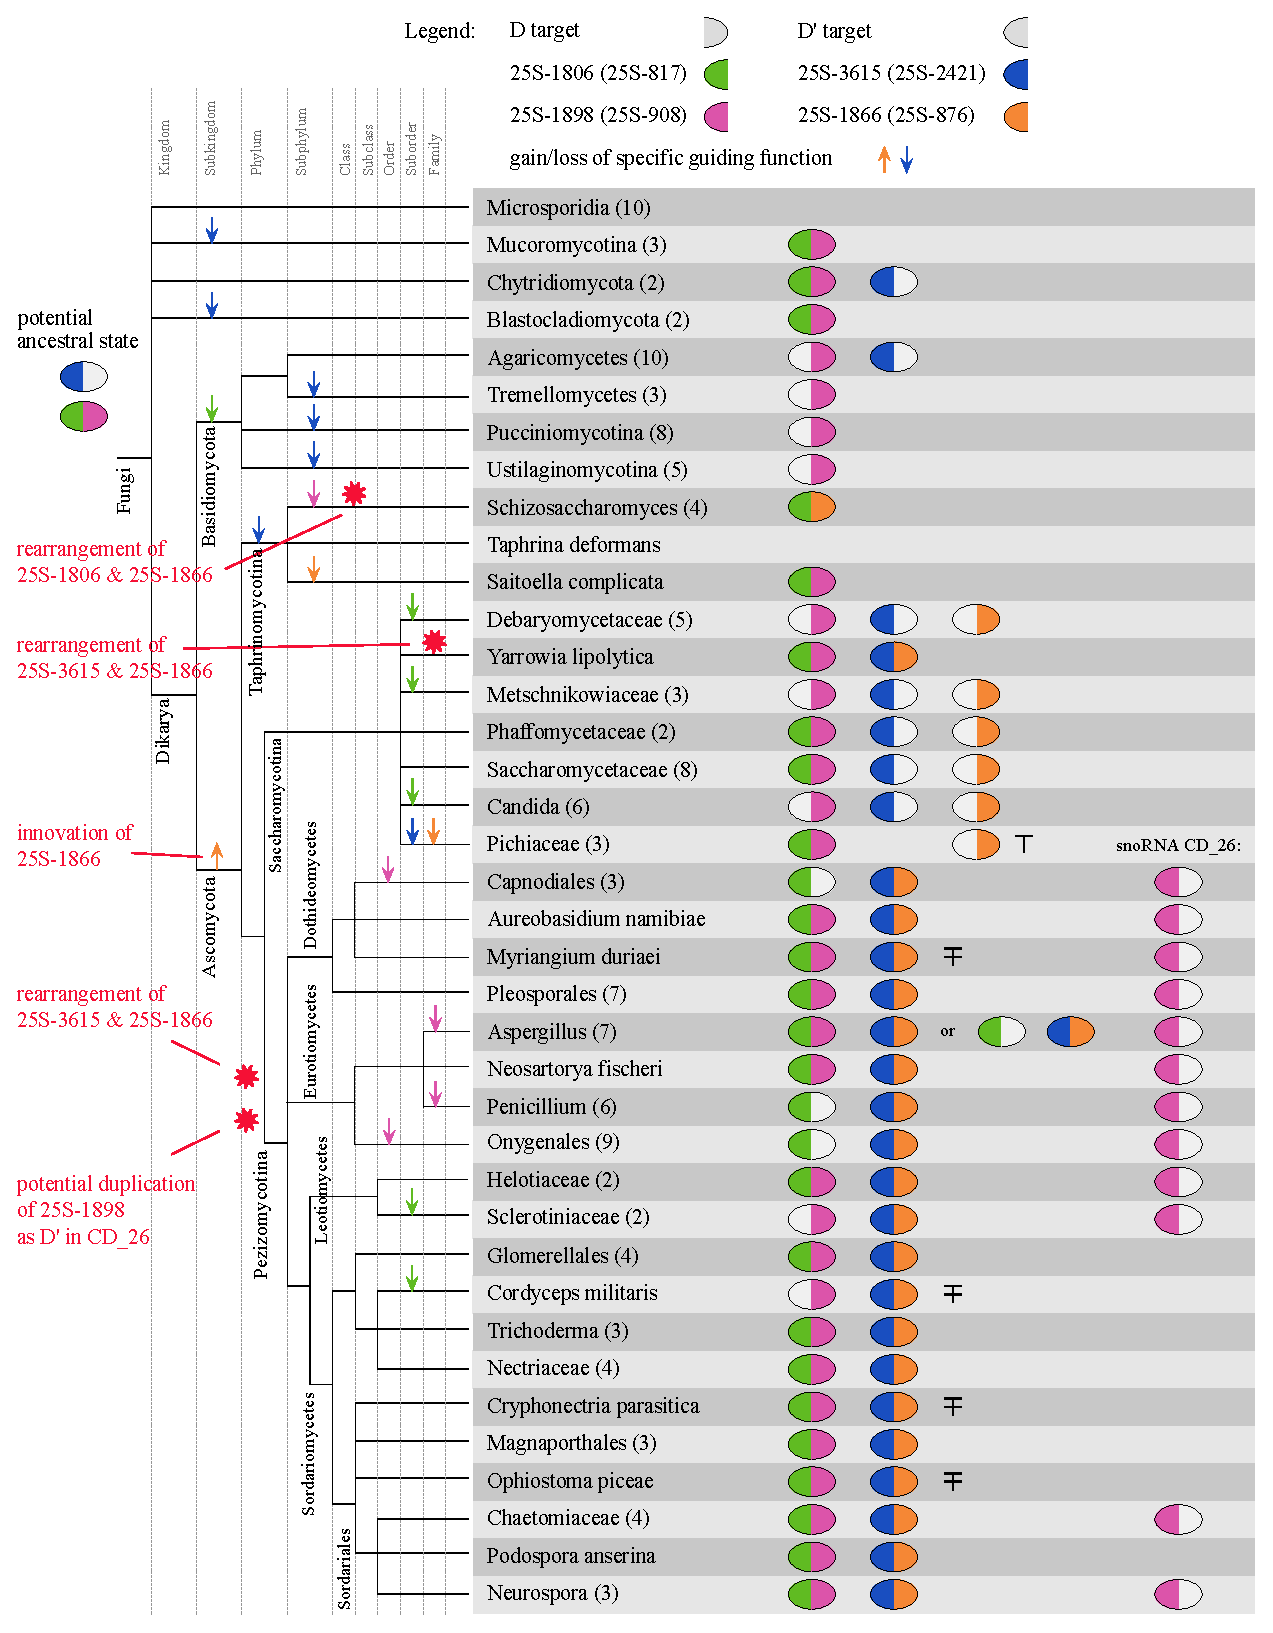
\includegraphics[width=0.9\textwidth]{pics/target_switches_CD_5.eps}
  \caption[Potential evolutionary history of \sno\ clan
  CD\_5.]{Potential evolutionary history of \sno\ clan CD\_5 involving
  four modification sites on the LSU rRNA. Gain/loss events
  are displayed with arrows, while potential rearrangements are shown
  with red stars. $\top$ 25S-1866 is solely found in Pichia. $\mp$ Putative since LSU sequences are missing; \sno s show convincing
ASE conservation.}
  \label{fig:CD_5}
\end{figure*}

\textbf{The \sno\ clan CD\_5} comprises three distinct budding yeast \sno\
sequences (snR60, snR72, and snR78) which at first sight do not share
a common evolutionary background. snR60 was verified to guide
methylations at 25S-1898 (single sequence 25S-908, D target) and
25S-1806 (25S-817, D' target), snR72 guides the methylation at
25S-1866 (25S-876, D target), and snR78 was shown to direct the
modification at position 25S-3615 (25S-2421, D' target). The
methylations at position 25S-1806, 25S-1898, and 25S-3915 map to known
and verified modifications in human large subunit ribosomal RNAs and
hence, are supposed to be ancient, which in consequence suggest the real existence
of both the methylations and the guiding snoRNAs at the root of fungi.
However, through individual target switches in the cause of fungal
evolution, the history of these sequences became connected. A
taxonomic tree displaying a potential evolutionary history involving
\sno s that are predicted to guide the above mentioned modifications is shown in
Figure \ref{fig:CD_5}. Therein, the putative ancient state is
described to be constituted of two individual \sno\
sequences guiding the three ancient methylations. 
Parsimonious deletion and innovation events of target interactions are marked
accordingly. The emergence of the fourth modification, 25S-1866, is
predicted at the root of Ascomycota, since all diverging
lineages are either predicted or verified to target this specific
site. The loss of any of the four guiding functions occurred rather
frequently in several lineages, e.g., Basidiomycota are supposed to
have lost the guiding potential for 25S-1806 while different
Basidiomycota lineages are further predicted to have lost the ability
to guide methylation at 25S-3615.

\begin{figure*}
  \centering
  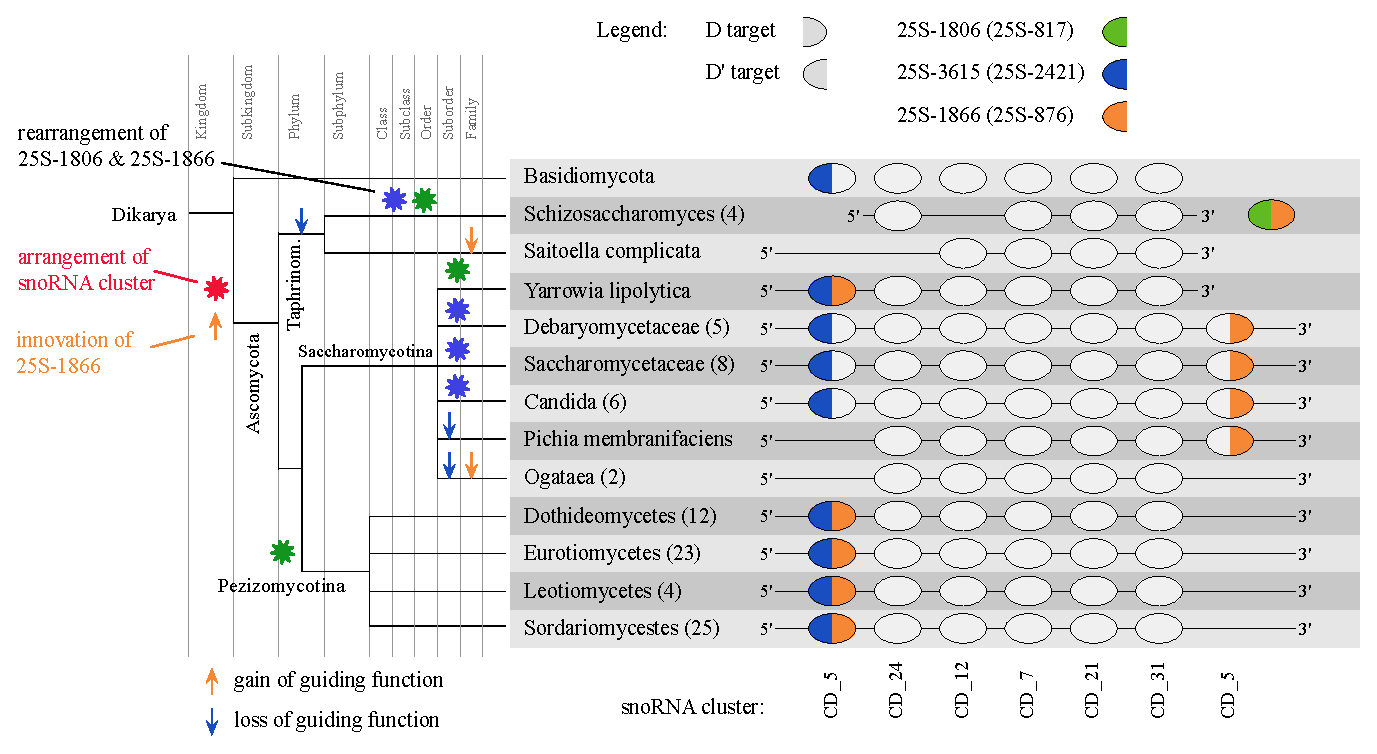
\includegraphics[width=\textwidth]{pics/target_switches_CD_5_cluster.eps}
  \caption[Evolution of a \sno\ cluster harboring CD\_5
  sequences.]{Sequences of the CD\_5 \sno\ family are incorporate into
  a polycistronic transcript that harbors up to seven \sno\
  genes. This cluster with its highly conserved structure and size occurred at the root of Ascomycota, but most of
  its genes arose at least at the root of Dikarya. There are different
  potential histories regarding the evolution of the cluster depending on how
  the newly innovated target guiding function at position 25S-1866
  (orange) was initially introduced in this polycistronic
  transcript. A) Evolutionary history under the assumption that
  25S-1866 is incorporated as a second guiding function into the \sno\
  guiding 25S-3615. B) History under the hypothesis that a novel
  single guide \sno\ is introduced at the 3' end of the \sno\
  cluster. The most parsimonious rearrangement events that led to the
  observed cluster organization are depicted in
  blue and green stars, according to hypothesis A and B, respectively.}
\label{fig:CD_5_cluster_history}
\end{figure*}

Besides such ordinary processes of gain and loss events, it happened
several times during fungal evolution that target interactions
of the mentioned four modifications switched between different \sno s.
It is a noteworthy fact that the actual target site within the \sno\
(D' or D target) are mostly preserved. Within the Taphrinomycotina
lineage, including the fission yeast, target guiding functions at
25S-1806 (D' target) and 25S-1866 (D target) are incorporated into one \sno\ sequence after
the original guidance of 25S-1898 (D target) went missing. 

At the root of Ascomycota, a polycistronic \sno\ transcript is
arranged including the \sno\ sequences of snR77 (CD\_24), snR76 (CD\_12),
snR75 (CD\_7), snR74 (CD\_21), and snR73 (CD\_31) in 5'-3' direction, see Figure
\ref{fig:CD_5_cluster_history}.  All these \sno\ families
are already present at the root of Dikarya, distributed over large
distances or different chromosomes. After the formation of this
cluster, the precise order and the
length of approx. 1.5kb is highly conserved throughout all
Ascomycota. 

It might have happened that a \sno\ of clan CD\_5 guiding
methylation at 25S-3615 is already present at the 5' end of this
cluster when it emerged. However, there are several possibilities how
the \sno\ cluster evolved after the innovation of guiding function for 25S-1866. 
One hypothesis (Blue stars in Figure \ref{fig:CD_5_cluster_history}) is the initial incorporation of 25S-1866 into the \sno\
that already guides 25S-3615, creating a double guide \sno at the 5'
end of the polycistronic transcript. In Taphrinomycotina, the loss of
guiding function for 25S-3915 and 25S-1898  might have caused the
rearrangement of the 25S-1806 and 25S-1866 and the exclusion from the
\sno\ cluster. At the root of Saccharomycotina, the double guide \sno\
might have split up leaving a single guide at the 5' end (25S-3615)
and a novel single guide at the 3' end of the cluster
(25S-1866). The original formation is solely conserved in
\Yli. In another hypothesis, evolution might have taken the other
way round (green stars in Figure
\ref{fig:CD_5_cluster_history}). Assuming the innovation of 25S-1866
led to a novel single guide \sno\ that is located at the 3' end of the
\sno\ cluster, as seen in Saccharomycetaceae, \yli\ would be the only
organism in Saccharomycotina where a  rearrangement is detected. In
result, the previously single guide sequences are reorganized into a
double guide sequence  with guiding ability for
25S-3615 as D' target and 25S-1866 as D target. This novel double guide is now located at the 5' end of the
cluster. 
Coincidentally, the same reorganization happened at the root
of Pezizomycotina, where the first \sno\ of the cluster is found to
guide modifications at position 25S-3615 (D') and 25S-1866
(D). Proteins that are located up- and downstream of the previously
described \sno\ cluster are not found to be conserved throughout major
fungal lineages.


A further interesting observation is the potential duplication of
target interaction for 25S-1898 at the root of Pezizomycotina. This
ability is inserted into family snR67 (CD\_26) as a D' target in the lineages
Dothideomycetes, Eurotiomycetes, and Leotiomycetes
(ICI$_{Pezizomycotina}$: 1.13, mean
mfe: -18.79). Neurospora species
are also predicted to guide this methylation with its Nc\_CD\_26 (CD\_26) \sno \cite{Liu:2009}. In reverse the
original D' target of snR67, 25S-3836, was abolished in these
organisms and is not found to be restored in any other \sno\ family.
Please also confer Figure \ref{fig:additional_targets} for more
detailed information of family CD\_26. The invention of redundant
guides would explain the findings that in some of these species the original target
site of 25S-1898 vanished in CD\_5 \sno s, e.g., in Capnodiales, some Aspergillus
organisms, or Onygenales. Families CD\_5 and CD\_26 are not merged due
to a switch of the ASE (from D in CD\_5 to D' in CD\_26). 
\SB{Think about this: Interestingly, in lineages where the original target 25S-3836 of CD\_26 is lost, there is no functional connection to the orginal snoRNA family anymore. This means organisms of such lineages have no functional target sitem either D or D' in common with organisms of other lineages in this particular family. They show clear sequence homology, meaning that they probably descend from one another. evolution of a new snoRNA family due to target shift??}





\paragraph{\textbf{Multiple Target Interactions}}
It might happen, that \sno\ families are not only convincingly
predicted to guide one specific target modification but two or even
more with the same ASE.
\begin{table}
  \caption{Summary on
    multiple target predictions of families snR40 (CD\_43) and snR70 (CD\_61) that are guided with the same ASE.}
  \label{tab:redundant_predictions}
  \begin{center}
    \begin{footnotesize}
      \begin{tabular}{c|c|c|c|c}
        &pos&ICI$_{sno}$&$\varnothing$
          mfe&\# ia\\
        \hline
        &18S-1400&0.95&-12.96&67/90\\
        \raisebox{1.5ex}[-1.5ex]{snR40}&18S-614&1.61&-21.96&71/90\\
        \hline
        &18S-1843&1.48&-17.82&86/102\\
        &5.8S-155&1.16&-12.99&92/102\\
        snR70&18S-348&1.04&-12.99&83/102\\
        &18S-1827&1.02&-12.49&85/102\\
        &5.8S-120&1.00&-11.36&91/102\\
      \end{tabular}
    \end{footnotesize}
  \end{center}
\end{table}
An outstanding example is given by \cd\ family
snR40 (CD\_43) which is predicted and experimentally validated to guide
methylation at position 18S-1400 (18S-1271) with its D' target binding
region. This interaction is predicted in 67 out of 90 \sno s and provides
an ICI score of 0.95 with a mean interaction energy of -12.96
kcal/mol. However, an even better target is predicted at position
18S-614 (18S-562) with an ICI score of 1.61 and a mean mfe of
-21.69. This interaction is found in 71 organisms. All 67 \sno s
predicted to guide the first target are also predicted to guide the
latter one, in a vast majority of cases even with a better binding
energy. But since the genuine modification is neither reported in
\sce, \ncr, or human, this prediction, albeit its overly convincing
nature, remains hypothetical. 

An even more vital example is provided by family snR70 (CD\_61) at its D' ASE.
Not less than five potential targets are predicted with an ICI score
above 1.0, a mean mfe below -11.30 and more than 80 single sequence
predictions. Details are shown in Table
\ref{tab:redundant_predictions}. This time, the most persuasive
prediction is experimentally confirmed, whereas the other predicted
positions were not shown to be modified yet. 
